%%%%%%%%%%%%%%%%%%%%%%%%%%%%%%  IEEEsample.tex
%%%%%%%%%%%%%%%%%%%%%%%%%%%%%%%%%%%%%%%%%
%%%%%%%%%%%%%%%%%%%%%%%    More information: see the header of IEEEtran.sty
%%%%%%%%%%%%%%%%%%%%%%%
%%%%%%%%%%%%%%%%%%%%%%%%%%%%%%%%%%%%%%%%%%%%%%%%%%%%%%%%%%%%%%%%%%%%%%%%%%%%%%%%
%%%%

\documentclass[10pt,twoside]{IEEEtran}
%\documentclass[conference]{IEEEtran}

%%%\IEEEoverridecommandlockouts

\usepackage[ruled,linesnumbered]{./algorithm2e}
%%for algorithm2e package, label has to be following caption in the same line!!!
\renewcommand{\algorithmcfname}{ALGORITHM}
\SetAlFnt{\small}
\SetAlCapFnt{\small}
\SetAlCapNameFnt{\small}
\SetAlCapHSkip{0pt}
\IncMargin{-\parindent}

%% \RequirePackage{times}
%% \RequirePackage{algorithmic}
%% \PassOptionsToPackage{boxed}{algorithm}
%% \RequirePackage{algorithm}
%% \RequirePackage{multicol}
%\renewcommand{\algorithmicrequire}{\textbf{Inputs:}}
%\renewcommand{\algorithmicensure}{\textbf{Outputs:}}
%\DeclareMathAlphabet{\mathtsl}{OT1}{ptm}{m}{sl}

%\def\BibTeX{{\rm B\kern-.05em{\sc i\kern-.025em b}\kern-.08em1
%    T\kern-.1667em\lower.7ex\hbox{E}\kern-.125emX}}

%\newtheorem{theorem}{Theorem}
%\newtheorem{lemma}{Lemma}
%\newtheorem{example}{Example}
%\newtheorem{corollary}{Corollary}

\RequirePackage{amssymb, mathptm}
\usepackage{amsbsy}
\usepackage{amsthm}
\usepackage{graphicx}
\usepackage{helvet}
\usepackage{enumerate}
\usepackage{amsmath}
\usepackage{amsfonts}
\usepackage{graphicx}
\usepackage{multirow}
\usepackage{subfig}
\usepackage{cases}
\usepackage{comment}



%%indent in algorithm


%\setcounter{page}{1}


% New command for the table notes.
\def\tabnote#1{{\small{#1}}}

% New command for the line spacing.
\newcommand{\ls}[1]
    {\dimen0=\fontdimen6\the\font
     \lineskip=#1\dimen0
     \advance\lineskip.5\fontdimen5\the\font
     \advance\lineskip-\dimen0
     \lineskiplimit=.9\lineskip
     \baselineskip=\lineskip
     \advance\baselineskip\dimen0
     \normallineskip\lineskip
     \normallineskiplimit\lineskiplimit
     \normalbaselineskip\baselineskip
     \ignorespaces
    }
%\renewcommand{\algorithmicrequire}{\textbf{Input:}}
%\renewcommand{\algorithmicensure}{\textbf{Output:}}

\newcommand{\beq}{\begin{equation}}
\newcommand{\eeq}{\end{equation}}
\newcommand{\beqarr}{\begin{eqnarray}}
\newcommand{\eeqarr}{\end{eqnarray}}
%\newcommand{\ov}{\overline}
\newcommand{\ov}{\bar}
\newcommand{\xor}{\bigoplus}
\newcommand{\Fm}{{\mathbb{F}}}



%the following is for space before and after align or other equation environment.

%%
\newtheorem{Algorithm}{Algorithm}[section]
\newtheorem{Definition}{Definition}[section]
\newtheorem{Example}{Example}[section]
\newtheorem{Proposition}{Proposition}[section]
\newtheorem{Lemma}{Lemma}[section]
\newtheorem{Theorem}{Theorem}[section]
\newtheorem{Corollary}{Corollary}[section]
\newtheorem{Conjecture}{Conjecture}[section]
\newtheorem{Problem}{Problem}[section]
\newtheorem{Notation}{Notation}[section]
\newtheorem{Setup}{Problem Setup}[section]

%%%

%%set spacing between table columns
\setlength{\tabcolsep}{3pt}

\begin{document}

%\thispagestyle{empty}
%\pagestyle{empty}

%\ls{1.5}

\title{\large{\textsc{Formal Verification of Sequential Galois Field Circuits using Word-Level FSM Traversal via Algebraic Geometry}}}
%\author{Tim Pruss\\
%A Master's Thesis Proposal\\
%Electrical \& Computer Engineering, University of Utah\\
%Spring Semester 2013
%}

\author{

\IEEEauthorblockN{Xiaojun Sun\IEEEauthorrefmark{1}, Priyank
  Kalla\IEEEauthorrefmark{1}, Florian Enescu\IEEEauthorrefmark{2}\\}
%\thanks{This work is sponsored in part by a grant from NSF \#CCF-546859.}
\IEEEauthorblockA{\IEEEauthorrefmark{1}Electrical \& Computer
  Engineering, University of Utah\\
\IEEEauthorrefmark{2}Mathematics \& Statistics, Georgia State
University \vspace{-0.25in}
 %\{lv, kalla\}@eng.utah.edu
}
%% \and
%% \IEEEauthorblockN{Florian Enescu\\} 
%% %\thanks{\normalsize  978-3-9810801-8-6/DATE12/$\copyright 2012$ EDAA}
%% \IEEEauthorblockA{Mathematics \& Statistics, Georgia State University
%% % fenescu@mathstat.gsu.edu
%% } 
}
 
\maketitle

%\markboth{MS Proposal by Tim Pruss}{}
\newcommand{\Fq}{{\mathbb{F}}_{q}}
\newcommand{\Fkk}{{\mathbb{F}}_{2^k}}
\newcommand{\Fkkx}[1][x]{\ensuremath{\mathbb{F}}_{2^k}[#1]\xspace}
\newcommand{\Grobner}{Gr\"{o}bner\xspace}
\newcommand{\B}{{\mathbb{B}}}
\newcommand{\Z}{{\mathbb{Z}}}
\newcommand{\F}{{\mathcal{F}}}
\newcommand{\G}{{\mathcal{G}}}
%%%

\newcommand{\debug}[1]{\textcolor{gray}{[ #1 ]}}


%\thispagestyle{empty}
%\pagestyle{empty}

%%%%%%%%%%%%%%%%%%%% Include your files here %%%%%%%%%%%%%%%%%%%%%
\begin{abstract}
Sequential circuits that implement Galois field arithmetic over
$\Fkk$ are prevalent in cryptography and error control coding, where
the datapath size $k$ is very large. Formal verification of sequential
arithmetic circuits with large datapath size is beyond the
capabilities of contemporary verification techniques. To address this
problem, this paper introduces a new concept of implicit state
enumeration of finite state machines (FSMs) performed at the
word-level. Using algebraic geometry, we show that the state-space of
a sequential circuit can be encoded, canonically, as solutions to a
multivariate word-level polynomial $\F(A)$ in $\Fkk$, where $A = {a_0,
\dots, a_{k-1}}$ represents the $k$-bit state-register (word). Subsequently,
the Groebner basis algorithm, along with elimination ideals and quotients 
of ideals can be employed for FSM traversal. We apply our approach 
to verify sequential Galois field multipliers with large datapath sizes, 
where contemporary techniques prove to be infeasible.
\end{abstract}

\section{Introduction}
Verification for sequential circuits has been extensively discussed for decade. Binary Decision Diagram (BDD) is the first
and most widely used canonical technique among those for sequential verification \cite{touati1990implicit}. It is easy to
manipulate any Boolean expressions with BDD and use them to enumerate implicit states. However, an issue that BDDs have to
face is the size explosion when Boolean variables increase significantly. Several modifications have been made to improve
this problem by optimizing original BDD \cite{gunther2001application} \cite{narayan1997reachability}, or by reducing Boolean
variables from circuits\cite{burch1991representing} \cite{jiang2003verification}. Some variants of BDD representation
have also been developed such as Linear Taylor Expansion Diagram (LTED) \cite{alizadeh2009sequential}.

Another sort of approaches are based on satisfiability theory (SAT). SAT-solver is applied to state space traversal and 
work through eliminations on Boolean constrains \cite{coudert1990verification}. By exploiting SAT-based algorithm, direct
reachability induction is proposed \cite{bjesse2000sat}. Still SAT-based approaches need to struggle with size explosion problem.

\section{Related Works}
G. Avrunin \cite{avrunin1996symbolic} introduced algebraic geometry into formal verification. In his paper, the corresponding
relation between varieties of ideals and circuit variables is discussed, and concepts such as intersect of varieties, ideal and
its generators and algebraic closure are explored. Yet, a self-contained system of algebraic geometry representation theory has
not been well-defined.

T. Pruss, el(which one should I cite?) developed a word-level abstraction method based on  Gr\"obner basis theory...

J. Lv, el (should I cite this part) gave out a F4-style reduction algorithm which can help speed up Gr\"obner basis calculation...


%\section{Review of Previous Work}
\label{sec:prev}

{\bf Canonical Decision Diagrams:} 
The Reduced Ordered Binary Decision Diagram
(ROBBD) \cite{BRYA86}, based on the Shannon's decomposition, was the
first significant contribution in this area. 
Motivated by the success of BDDs, 
variants of the Shannon's decomposition principle (Davio,
Reed-Muller, etc.) were explored to develop other functional decision
diagrams: FDDs \cite{okfdd}, ADDs \cite{add}, %MTBDDs\cite{mtbdd},  
HDDs \cite{hdd} and EVBDDs \cite{evbdd}. 
%While these are %{\it curiously} still 
%referred to as {\it Word-Level Decision Diagrams} \cite{WLS}, 
Binary Moment Diagrams (BMDs) \cite{bmd}, and its derivative K*BMDs
\cite{kbmd}, % and *PHDDs \cite{phdd}, 
depart from the Boolean
decomposition and perform the decomposition of a {\it linear} function
based on its two moments. The decomposition is still point-wise,
binary, w.r.t. each Boolean variable; these do not
serve the purpose of word-level abstraction from bit-level
representations. 

%% BMDs provide a compact representation for
%% integer arithmetic circuits such as multipliers and squarers. However,
%% these are inapplicable for modulo-arithmetic circuits over Galois fields.
%in our application, we encounter modulo-arithmetic circuits and that
%too over Galois fields. For such applications, these representations
%are inapplicable. Taylor Expansion Diagrams (TEDs) \cite{ted_tcomp}
%generalize the linear moment decomposition of BMDs into a Taylor
%series expansion --- this allows the representation of RTL
%descriptions as polynomials over bit-vectors. However, 
Taylor Expansion Diagrams (TEDs) \cite{ted_tcomp} are a word-level
canonical representation of a {\it polynomial expression}, but they do
not represent a {\it polynomial function} canonically. 
%For example, $f_1 = 0$ and $f_2 = 2x^2 - 2x
%\pmod{ 4}$ are two different polynomial representations of the zero
%function over $\Z_4$; but they are symbolically different
%polynomials and they have different (non-isomorphic) TED DAGs. 
While \cite{shekhar:tcad07}  and \cite{alizadeh:tcad2010} provide
canonical representations of polynomial functions, they do so over
$\Z_{2^k}$ and not over $\Fkk$.
%finite integer rings and not over Galois fields.  


MODDs \cite{modd} \cite{modd_tcomp} are a DAG representation of the
characteristic function of a circuit over Galois fields $\Fkk$. MODDs
come very close to satisfying our requirements as a canonical
word-level representation that can be employed over Galois fields, as
it essentially interpolates a polynomial from the characteristic 
function. However, MODDs do not scale very well for large circuits ---
this is because every node in the DAG can have up to $k$ children and
the normalization operations are very complicated for MODDs. They 
suffer from the size explosion problem during intermediate
computations. They are known to be infeasible beyond
32-bit circuits.  

%In the realm of theorem-proving and SMT-solving, many automated
%decision procedures have been devised that can decide
%satisfiability/validity of word-level formulas represented by a
%combination of theories, but they do not provide a canonical
%representation of the function implemented by a ``bit-blasted''
%circuit. 

{\bf Verification of Galois field circuits:} 
%% Symbolic computer algebra techniques have been employed for formal
%% verification of circuits over $\Z_{2^k}$ and also over $\Fkk$. 
%% %% The work of \cite{gao:gf-gb-ms} shows how to use Gr\"obner basis
%% %% techniques to count the zeros of an ideal $J$ over ${\mathbb{F}}_q$
%% %% (i.e. count $V_{{\mathbb{F}}_q}(J)$). The authors then follow-up with
%% %% an approach for {\it quantifier elimination} over Galois fields
%% %% ${\mathbb{F}}_q$ \cite{gao:qe-gf-gb}. While the above works present
%% %% the theory and algorithms, efficiency/improvements in Gr\"obner basis
%% %% computation is not addressed. So is also the case with other general
%% %% verification techniques using Gr\"obner bases \cite{Avrunin:CAV}
%% %% \cite{gbverify:2007} \cite{manna:program}, etc. 
%% The paper \cite{wienand:cav08} addresses verification of
%% finite-precision integer datapath circuits using the concepts of
%% Gr\"obner bases over the ring ${\mathbb{Z}}_{2^k}$. 
%% %They model the
%% %circuit constraints by way of arithmetic-bit-level (ABL) polynomials
%% %($\{G\}$) and formulate the verification test as an equivalent
%% %{\it variety subset problem}. To solve this, first they derive a term
%% %order to represent the circuit polynomials $\{G\}$ with a Gr\"obner
%% %basis. Then they compute a normal form $f$ of the specification $g$
%% %w.r.t. $\{G\}$. They show that, under certain constraints that are
%% %satisfied by their term order, the circuit is correct if and only if
%% %$f$ is a vanishing polynomial over ${\mathbb{Z}}_{2^k}$
%% %\cite{shekhar:tcad07}. 
%% In \cite{wedler:date11}, the authors further
%% show an integration of their approach within an SMT-solver for
%% arithmetic instances.  
%% %show that  the vanishing polynomial test can be
%% %omitted by formulating the problem directly over $Q :=
%% %{\mathbb{Z}}_{2^k} [X]/\langle x^2-x : x \in X \rangle$. 
In %\cite{ibm:ecc-ita11} \cite{blueveri:ita} 
\cite{ibm:blueveri},
%from IBM needs special mention: T
the authors present the {\sc BLUEVERI} tool from IBM for verification
of Galois field circuits for error correcting codes against an
algorithmic spec. The implementation consists of a set of
(pre-designed and verified) circuit blocks that are interconnected to
form the error correcting system. The spec is given as a set of design
constraints on a ``check file''. Their objective is to prove the 
equivalence of the implementation against this check file,
%They model
%the verification instance as a data-flow graph, represent each
%sub-circuit block with its known (word-level) polynomial over $\Fq$,
%and formulate the verification problem using the {\it Weak
%  Nullstellensatz} --- i.e. to check if the {\it variety} of the
%algebraic system ``{\it spec} $\neq$ {\it implementation}'' is empty
for which they employ a Nullstellensatz formulation.
%for which they use a Gr\"obner basis engine. 
%Their main
%contributions are: i) a ``term re-writing'' to specify the algorithmic
%description using polynomials (ideal); and ii) integrating an
%AIG-style \cite{AIG:2002} Boolean solver with their word-level
%decision procedure, with lazy signal computations and Boolean
%reasoning. 
For final verification, the polynomial system is given
to a computer algebra tool ({\sc Singular} \cite{DGPS}) to {\it
  compute} a reduced Gr\"obner basis. However, improvements to the
core Gr\"obner basis computational engine are not the subject of their
work.   

In %\cite{lv:phd} 
\cite{lv:date2012} 
%\cite{lv:hldvt2011} \cite{lv:vlsi2012}, 
{\it Lv et al.} present computer algebra
techniques for formal verification of Galois field arithmetic
circuits. Given a specification polynomial $f$, and a circuit $C$,
they formulate the verification problems as an ideal membership test
using the Strong Nullstellensatz and Gr\"obner bases. In \cite{lv:date2012}, the
authors show that for any combinational circuit, {\it there exists
a term order $>_1$ that renders the set of polynomials of the circuit
itself a Gr\"obner basis --- and this term order can be easily derived
by performing a topological traversal of the circuit}. By exploiting
this term order, verification can be significantly scaled
to $163$-bit (NIST-specified) cryptography circuits. 
In contrast to the work of \cite{lv:date2012}, we are not given a
specification polynomial. Given the circuit $C$, we want
to derive (extract) the word-level specification $f$. 
In this work, we build upon the results of
%\cite{gao:gf-gb-ms} \cite{gao:qe-gf-gb} %\cite{modd_tcomp} 
\cite{lv:date2012}. 

{\bf Polynomial Interpolation in Symbolic Computation:}
The problem of polynomial interpolation is a fundamental problem in
symbolic and algebraic computing which finds application in modular
algorithms, such as the GCD computation and polynomial
factorization. The problem is stated as follows: Given $n$ distinct
data points $x_1, \dots, x_n$, and their evaluations at these points
$y_1, \dots, y_n$,  {\it interpolate} a polynomial $\F(X)$ of degree
$n-1$ (or less) such that $\F(x_i) = y_i$ for $1 \leq i \leq n$. 
Let $t$ be the number of non-zero terms in $\F$ and let $T$ be the
total number of possible terms. When ${{t} \over {T}} << 1$, the
polynomial $\F$ is {\it sparse}, otherwise it is {\it dense}. Much of
the work in polynomial interpolation addresses sparse 
interpolation using the ``black-box'' model (also called the
algebraic circuit model) as shown in Fig. \ref{fig:blackbox}. 

\begin{figure}[hbt]
\centerline{
%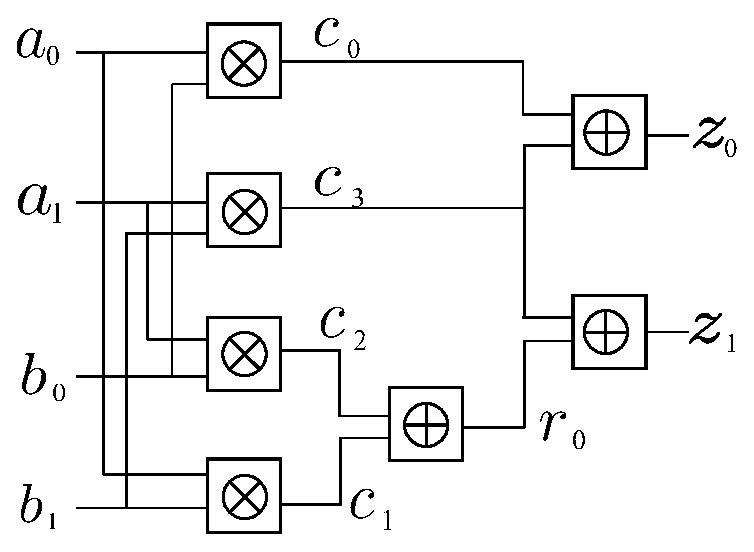
\includegraphics[scale=0.3]{../figures/2bitmultiplier.eps}
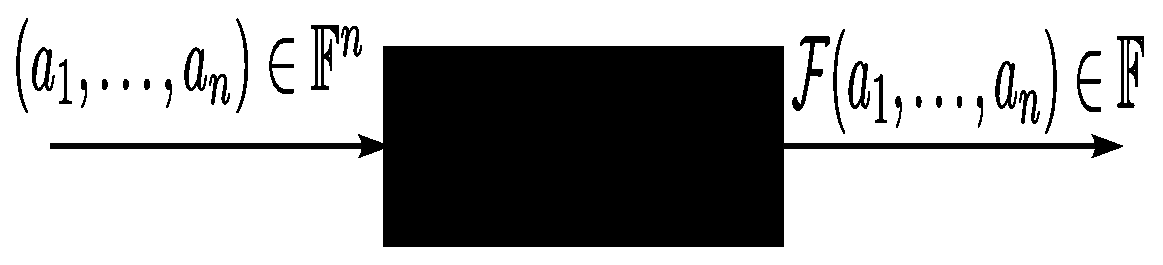
\includegraphics[scale=0.35]{../blackbox.eps}
}
\caption{The black-box or the algebraic circuit representation.}
\label{fig:blackbox}
\end{figure}

Let $\F$ be a multivariate polynomial in $n$ variables $\{x_1, \dots,
x_n\}$, with $t$ non-zero terms ($0 < t < T$), represented with a
black-box $B$. On input $(x_1, \dots, x_n)$,
the black-box evaluates $y_i = \F(x_1, \dots, x_n)$. Given also a
degree bound $d$ on $\F$, the goal is to interpolate the polynomial
$\F$ with a minimum number of {\it probes} to the black-box. The early
work of Zippel \cite{zippel:interpolate} and
Ben-Or/Tiwari \cite{ben-or-tiwari:interpolate} require $O(ndt)$ and
$O(T \log n)$ probes, respectively, to the black-box. These bounds
have since been improved significantly; the recent algorithm of
\cite{monagan:interpolate} interpolates with $O(nt)$ probes.  

Our problem falls into the category of {\it dense} interpolation, as
we require a polynomial that describes the function at each of the $q$
points of the field $\Fq$. Newton's dense interpolation technique,
with the black-box model, bounds the number of probes by $(d+1)^n$ ---
which  exhibits very high complexity. In the logic synthesis area, the
work of \cite{zilic:interpolate} investigates dense interpolation. Due
to the inherent high-complexity, their approach is feasible only for
applications over small fields, {\it e.g.} computing  Reed-Muller
forms for multi-valued logic.  

We can also employ the black-box model by replacing the black-box
(algebraic circuit) by the given circuit $C$; then every {\it probe}
of the black-box would correspond to a {\it simulation of the
  circuit}. As we desire a polynomial representation of the entire
function, exhaustive simulation would be required, which is
infeasible. Therefore, we propose a {\it symbolic approach} to
polynomial interpolation from a circuit using the Gr\"obner basis
computation. 
%It can be shown that the computational complexity of
%computing a Gr\"obner basis for our problem, in the worst case, is
%$q^{O(n)}$, where $q = 2^k$, $k$ is the datapath width and $n$ is the
%number of variables in the circuit.  

%\section{Galois Fields, Polynomial Functions \& Hardware Design}
\label{sec:prelimgf}
%\vspace{-0.035in}

%% We briefly describe the relevant concepts related to Galois fields
%% $\Fkk$; for more details, interested readers may refer to the textbook 
%% \cite{galois_field:mceliece}. 
%% %to put the complexity of the verification problem in perspective, 
%% %to shed some light on the complexity of our design verification, 
%% We also review some VLSI architectures used for Galois field
%% computations \cite{mastro:phd} \cite{acar:1998} \cite{wu:2002}
%% \cite{Knezevic:2008} \cite{eccld} \cite{ecc163}. In our experiments,
%% we have verified custom designs based on these architectures. 

%%%%%%%%%%%%%%%%%%%%%%%%%%%%%%%%%%%%%%%%%%%%%%%%%%%%%%%%%%%%%%%%%%%%%%%%%%%%
%% %\begin{Definition}
%% A finite field, also called a {\bf Galois field}, denoted by $F_q$, is
%% a set of $q$ elements, including two distinguished elements 0 and 1,
%% along with operations $'+'$ and $'\cdot'$ (addition and
%% multiplication) that satisfy the following properties: 
%% \begin{itemize}
%% \item ($F_q, +, 0$) forms an Abelian group.

%% % \begin{itemize}
%% % \item  Closure: $\forall a, b \in F_q, a + b \in F_q$.
%% % \item Associativity: $\forall a, b, c \in F_q, a+(b+c)=(a+b)+c$.
%% % \item Commutativity: $\forall a, b \in F_q, a+b=b+a$.
%% % \item Additive Identity: $\forall a \in F_q, a+0=a$. 
%% % \item Additive Inverse: $\forall a \in F_q$, there is an additive
%% %   inverse element $-a \in F_q$ such that $a+(-a)=0$. 
%% %\end{itemize}

%% \item ($F_q, +, \cdot, 0, 1$) forms a commutative ring with unity.
%% % \begin{itemize}
%% % \item Multiplication closure: $\forall a, b \in F_q, a \cdot b \in
%% %   F_q$.
%% % \item Multiplication Associativity: $\forall a, b, c \in F_q, a \cdot
%% %   (b \cdot c)=(a \cdot b)\cdot c$.  
%% % \item Multiplication Commutativity: $\forall a, b \in F_q, a \cdot b=b \cdot a$. 
%% % \item Multiplication Identity: $\forall a \in F_q, a\cdot 1=a$. 
%% % \item Distributivity: $\forall a, b, c \in F_q, a \cdot (b+c)=(a
%% % \cdot b)+(a \cdot c)$. 
%% % \end{itemize}

%% \item Every non-zero element in $F_q$ has a   multiplicative inverse:
%%   $\forall a \in F_q - \{0\}, \exists a^{-1} \in F_q$ such that $a \cdot
%%   a^{-1}=1$. 

%% \item The number of elements $q$ of the finite field is a
%%   power of a prime integer, i.e. $q = p^k, k \geq 1, p=$ prime. 

%% \end{itemize}
%% %\end{Definition}

A Galois field $\Fq$ is a field with a finite number of elements. The
number of elements $q$ of the field is a power of a prime integer ---
i.e. $q = p^k$, where $p$ is a prime integer, and $k \geq 1$
\cite{galois_field:mceliece}. 
%Galois fields are denoted as ${\mathbb{F}}_{q}$ and also $GF(q
%=p^k)$. 
We are interested in fields where $p = 2$ and $k >1$ --- i.e. {\it
  binary Galois extension   fields} $\mathbb{F}_{2^k}$ --- as they are
widely employed in hardware implementations of cryptography
primitives.  

To construct ${\mathbb{F}}_{2^k}$, we take the polynomial ring
${\mathbb{F}}_2[x]$, where ${\mathbb{F}}_{2} = \{0, 1\}$, and an
irreducible  polynomial $P(x) \in {\mathbb{F}}_2[x]$ of degree $k$, and
construct ${\mathbb{F}}_{2^k}$ as ${\mathbb{F}}_2[x] \pmod{   P(x)}$. As a
result, all field operations are performed 
modulo the irreducible polynomial $P(x)$ and the coefficients are
reduced modulo $p=2$. %=2$; due to which $-1 = +1$ over $\Fkk$. 
Any element $A \in {\mathbb{F}}_{2^k}$ can be represented in polynomial
form as $A = a_0 +  a_1 \alpha + \dots + a_{k-1} \alpha^{k-1}$, where
$a_i \in {\mathbb{F}}_2, i = 0, \dots, k-1$, and $\alpha$ is the root of
the irreducible polynomial, {\it i.e.} $P(\alpha)=0$. 
%The field
%$\Fkk$ can therefore be construed as a $k$-dimensional vector space
%over ${\mathbb{F}}_2$.

%For
%example, $\mathbb{F}_{16} =  \mathbb{F}_2[x] \pmod{ x^4 + x + 1}$. 

%% \debug{
%% The {\it characteristic} of any finite field with
%% unity element $1$ is the least integer $n$ such that $1 + \dots + 1$
%% {\it (n times)} $= 0$. The characteristic of fields of the type
%% ${\mathbb{F}}_{p^k}$ %{\mathbb{F}}_p[x] \pmod{ P(x)}$ 
%% is the prime integer $p$. Since in our
%% case $p = 2$, all fields of the type $\Fkk$, for any given $k$, have 
%% characteristic 2. As a result, all field operations are performed
%% modulo the irreducible polynomial $P(x)$ and the coefficients are
%% reduced modulo $p=2$; due to which $-1 = +1$ over $\Fkk$. 
%% }

%% Any element $A \in \mathbb{F}_{2^k}$ can be represented in polynomial
%% form as $A = a_0 +  a_1 \alpha + \dots + a_{k-1} \alpha^{k-1}$, where
%% $a_i \in \mathbb{F}_2, i = 0, \dots, k-1$, and $\alpha$ is the root of
%% the irreducible polynomial, {\it i.e.} $P(\alpha)=0$. The field
%% $\Fkk$ can therefore be construed as a $k$-dimensional vector space
%% over $\mathbb{F}_2$.



\begin{Example}\label{ex:1}
{\it
Let us construct ${\mathbb{F}}_{2^4}$ as ${\mathbb{F}}_2[x] \pmod{
  P(x)}$, where $P(x)=x^4+x^3+1 \in {\mathbb{F}}_2[x]$ is an
irreducible polynomial of degree $k =4$. Let $\alpha$ be the root of
$P(x)$, i.e. $P(\alpha)=0$.  Any element $A \in {\mathbb{F}}_2[x]
\pmod{ x^4 + x^3 + 1}$ has a representation of the type: $A = a_3 x^3
+ a_2 x^2 +  a_1 x + a_0$ where the coefficients $a_3, \dots, a_0$ are
in ${\mathbb{F}}_2 = \{0, 1\}$. Since there are only 16 such
polynomials, we obtain 16 elements in the field
${\mathbb{F}}_{16}$. Each element in can then be viewed as a 4-bit
vector over ${\mathbb{F}}_2$: ${\mathbb{F}}_{16}=\{(0000),(0001),
\dots (1110),(1111)\}$.  Each element also has an exponential
representation; all three representations are shown in Table
\ref{tab:gfelement}. For example, consider the element $\alpha^{12}$.
Computing $\alpha^{12} \pmod{ \alpha^4+\alpha^3+1} = \alpha + 1
= (0011)$; hence we have the three equivalent representations. 
}

\vspace{-0.1in}
\begin{table}[h]
\begin{center}
{\tiny
\caption{Bit-vector, Exponential and Polynomial representation of
elements in  ${\mathbb{F}}_{2^4} = {\mathbb{F}}_2[x]
\pmod{x^4+x^3+1}$}\label{tab:gfelement}  
\begin{tabular}{|c|c|c||c|c|c|} 
\hline
$a_3a_2a_1a_0$ & Exponential & Polynomial     &$a_3a_2a_1a_0$ & Exponential & Polynomial  \\
\hline
$0000$        & $0$         & $0$            & $1000$ & $\alpha^3$ &  $\alpha^3$\\
\hline
$0001$        & $1$         & $1$            & $1001$ & $\alpha^4$ & $\alpha^3 + 1$\\
\hline
$0010$        & $\alpha$    & $\alpha$       & $1010$ & $\alpha^{10}$&$\alpha^3 + \alpha$  \\
\hline
$0011$        & $\alpha^{12}$& $\alpha + 1$   & $1011$ & $\alpha^5$ & $\alpha^3+\alpha+1$\\
\hline
$0100$        & $\alpha^2$  & $\alpha^2$     &  $1100$ & $\alpha^{14}$ & $\alpha^3 + \alpha^2$\\
\hline
$0101$        & $\alpha^9$   &$\alpha^2 + 1$ & $1101$  &$\alpha^{11}$  & $\alpha^3+\alpha^2+1$\\
\hline
$0110$        & $\alpha^{13}$& $\alpha^2 + \alpha$ & $1110$ & $\alpha^8$& $\alpha^3+\alpha^2+\alpha$\\
\hline
$0111$        &$\alpha^7 $ & $\alpha^2+\alpha+1$ & $1111$ &$\alpha^6$ & $\alpha^3+\alpha^2+\alpha+1$\\
\hline
\end{tabular}
}
\end{center}
\end{table}
\end{Example}




%%%%%%%%%
{\bf Polynomial Functions $f: \Fkk \rightarrow \Fkk$:} 
Arbitrary mappings among $k$-bit vectors can be constructed; each such
mapping generates a function $f: \B^k \rightarrow \B^k$. 
%. Since every
%$k$-bit vector can be construed as an element in $\Fkk$ (as shown in
%the above example), every such function corresponds to a function over
Every such function is also a polynomial function over Galois fields:
$f: \Fkk \rightarrow \Fkk$.  

\begin{Theorem}
From \cite{ff:1997}: 
Any  function $f: \Fq \to \Fq$ is a polynomial function
over $\Fq$, that is there exists a polynomial $\F \in \Fq [x]$ such
  that $f(a) = \F(a)$, for all $a \in \Fq$. 
\end{Theorem}

By analyzing $f$ over each of the $q$ points, one can apply
{\bf Langrange's interpolation formula} and interpolate a polynomial
$\F(x) = \sum_{k=1} ^q  \frac{ \prod_{i \neq k}  (x -x_i)}{\prod_{i \neq k}
  (x_k -x_i)} \cdot f(x_k)$, which is a polynomial of degree at 
most $q-1$ in $x$. One can easily see that $\F(a)=f(a)$ for all $a \in
\Fq$, and $\F(x)$ is therefore the polynomial function representation
of $f$. 

%% \begin{Example} {\it
%% Let $A = \{a_2, a_1, a_0\}$ and $Y = \{y_2, y_1,
%% y_0\}$ be 3-bit vectors.  Consider the function $Y[2:0] = A[2:0]
%% >> 1$, i.e. a {\bf bit-vector right shift} operation on $A$. 
%% The function maps as follows:

%% \begin{center}
%% {\small
%% \begin{tabular}{c|ccc|c||c|ccc|c}
%% $\{a_2a_1a_0\}$  & $A$ &$\rightarrow$& $\{y_2y_1y_0\}$ &$Y$ &
%%   $\{a_2a_1a_0\}$  &$A$&$\rightarrow$& $\{y_2y_1y_0\}$ &$Y$\\
%% \hline
%% 000  &0 &$\rightarrow$& 000 & 0 & 100  &$\alpha^2$ &$\rightarrow$& 010 &  $\alpha$ \\
%% 001  &1 &$\rightarrow$& 000 & 0 & 101  &$\alpha^2 + 1$ &$\rightarrow$&010 & $\alpha$ \\
%% 010  &$\alpha$ & $\rightarrow$ & 001& 1 & 110  &$\alpha^2 + \alpha$&$\rightarrow$& 011 &$\alpha + 1$ \\   
%% 011  &$\alpha + 1$ &$\rightarrow$& 001 &1 & 111& $\alpha^2 + \alpha + 1$ &$\rightarrow$& 011 &$\alpha + 1$\\
%% \hline
%% \end {tabular}
%% }
%% \end{center}

%% If we model this function as $f: {\mathbb{Z}}_{8} \rightarrow
%% {\mathbb{Z}}_{8}$, then using the results of \cite{singmaster}
%% \cite{chen_95} \cite{chen_96}, we deduce that this function is not a
%% polynomial function over ${\mathbb{Z}}_{8}$. However, applying
%% Largange's interpolation formula over ${\mathbb{F}}_{2^3}$, we obtain
%% the following polynomial function representation, $Y =
%% (\alpha^2+1)A^4+(\alpha^2+1)A^2$, where $P(\alpha) = \alpha^3 +
%% \alpha + 1 = 0$. 
%% }
%% \end{Example}

An important property of Galois fields is that for all elements $A \in
{\mathbb{F}}_q, A^q = A$, and hence $A^q - A =  0.$ Therefore, the
polynomial $x^q -x$ {\it vanishes} on all points in
$\Fq$. Consequently, any polynomial $\F(X)$ can be reduced $\pmod{ X^q
  - X}$ to obtain a canonical representation $\F(X) \pmod{X^q - X}$
with degree at most $q-1$. 
%Such {\it vanishing polynomials} will form
%an important part of our formulation.  

\begin{Definition}
Any function $f: \Fq^d \to \Fq$ has a unique canonical representation
(UCR) as polynomial $\F \in \Fq[x_1,\dots, x_d]$ such that all its 
nonzero monomials are of the form $x_1^{i_1}\cdots x_d^{i_d}$ where $0
\leq i_j \leq q-1$, for all $j=1, \ldots d$.
\end{Definition}


\subsection{Hardware Implementations of Galois Field Arithmetic}
% Operations Over $\mathbb{F}_{2^k}$}

{\bf Point Addition over Elliptic Curves:} The main operations of
encryption, decryption and authentication in elliptic curve
cryptography (ECC) rely on {\it point additions} and {\it doubling}
operations on elliptic curves designed over Galois fields. 
%Point multiplication involves a series of addition and doubling of
%points on the elliptic curve. % -- this, in turn, requires finite
%field multiplications.  
%A drawback of traditional approaches is that they require
%point multiplication is that each point addition and doubling 
In general, this requires computation of multiplicative inverses over
the field - which is expensive. Modern approaches represent
the points in projective coordinate systems, {\it e.g.}, the
L$\acute{o}$pez-Dahab (LD) projective coordinate \cite{eccld},
%\cite{ecc:software},
which eliminates the need for multiplicative inverses and improves the
efficiency of these operations. 

%%%

%% \begin{Example}
%% {\it 
%% Consider point addition in L$\acute{o}$pez-Dahab (LD) projective
%% coordinate. Given an elliptic curve: $Y^2 + XYZ = X^3Z + aX^2Z^2 +
%% bZ^4$ over $\mathbb{F}_{2^k}$,   where $X,Y,Z$ are $k$-bit vectors
%% that are elements in $\mathbb{F}_{2^k}$ and similarly, $a, b$ are
%% constants from the field.   Let ($X_3$, $Y_3$, $Z_3$) = ($X_1$, $Y_1$,
%% $Z_1$) + ($X_2$, $Y_2$, $1$)  represent point addition over the
%% elliptic curve.  Then $X_3$, $Y_3$, $Z_3$ can be computed as follows: 

%% \begin{align*}
%% A &= Y_2 \cdot Z_1^2 + Y_1 \\
%% B &= X_2 \cdot Z_1 + X_1 \\
%% C &= Z_1 \cdot B \\
%% D &= B^2 \cdot(C + a Z_1^2) \\
%% Z_3 &= C^2 \\
%% E &= A \cdot C  \\
%% X_3 &= A^2 + D + E  \\
%% F &= X_3 + X_2 \cdot Z_3 \\
%% G &= X_3 + Y_2\cdot Z_3 \\
%% Y_3 &= E\cdot F + Z_3 \cdot G \\
%% \end{align*}
%% }
%% \end{Example}

\begin{Example}
{\it 
Consider point doubling in LD projective coordinate system. Given an
elliptic curve: $Y^2 + XYZ = X^3Z + aX^2Z^2 + bZ^4$.  
Let  ($X_3$, $Y_3$, $Z_3$) = 2($X_1$, $Y_1$, $Z_1$), then $X_3, Y_3,
Z_3$ can be computed as: $X_3 = X_1^4 + b \cdot Z_1^4; ~~Z_3 = X_1^2
\cdot Z_1^2; ~~Y_3 = b Z_1^4 \cdot Z_3 + X_3 \cdot (aZ_3 + Y_1^2 +
bZ_1^4 )$. 
}
\end{Example}

The multiplication and iterative squaring operations in the above
computation are usually implemented using custom-designed Galois field
multipliers, such as the Mastrovito \cite{mastro:1989}, Montgomery
\cite{acar:1998}, Barrett multipliers \cite{Knezevic:2008}, or
composite-field multipliers \cite{cfmulti:1996} --- which are, in
turn, hierarchically designed.  
For example, Montgomery reduction (MR)
computes: $MR(A,B)=A\cdot B \cdot R^{-1} \pmod {P(x)}$, 
where $A,B$ are $k$-bit inputs, $R$ is suitably chosen as
$R={\alpha}^k$, $R^{-1}$ is multiplicative inverse of $R$ in
${\mathbb{F}}_{2^k}$, and $P(x)$ is the irreducible polynomial.
Since Montgomery reduction cannot directly compute $A\cdot B \pmod
{P(x)}$, we need to pre-compute $A\cdot R$ and $B\cdot R$, as shown in
Figure \ref{fig:mm4}.   

\begin{figure}[hbt]
	\begin{center}
	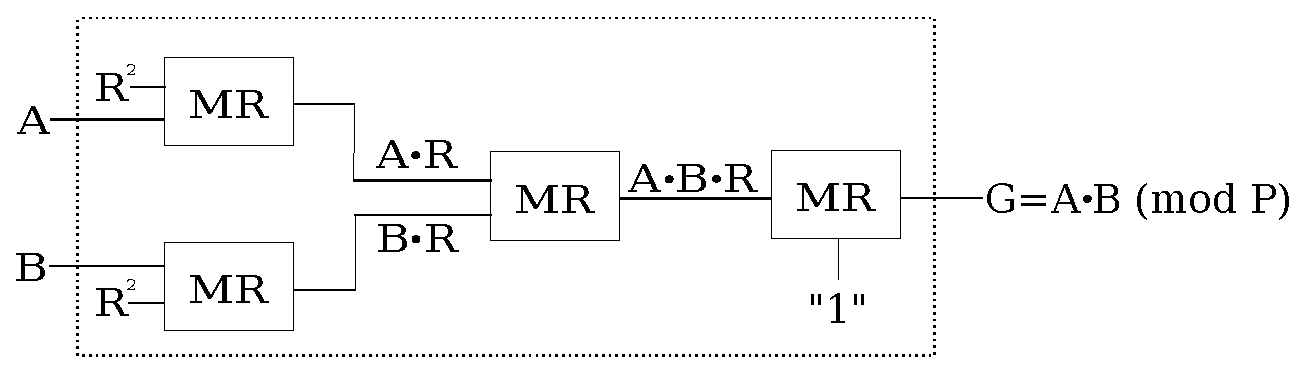
\includegraphics[scale=0.4]{../new_mmcircuit.eps}
	\end{center}
	\caption{{\it Montgomery} multiplication over $\mathbb{F}_{2^k}$
          using four Montgomery reductions.}
	\label{fig:mm4}
\end{figure}

Given a hierarchically designed Montgomery multiplier, we will first
extract polynomials $AR, BR, ABR$ from the sub-circuit blocks. By
analyzing the interconnection of these sub-circuits at word-level, we
can then apply our approach at a higher-level, to extract the function
of the entire circuit. Performing such operations hierarchically, we
will apply our approach to reverse-engineer point-addition circuits
designed using a variety of such Galois field adder and multiplier
circuits.  

%\section{Computer Algebra Preliminaries}
\label{sec:ideals}

%We review basic commutative algebra concepts related
%to ideals, varieties, Nullstellensatz and Gr\"obner bases, and their 
%application over Galois fields; the material is referred from
%\cite{ideals:book} \cite{gb_book} and \cite{gao:gf-gb-ms}. 

We denote a Galois field of $q$ elements by $\Fq$, where $q = 2^k$ in
our case. Let $\Fq[x_1,\dots, x_d]$ be
the polynomial ring over $\Fq$ with indeterminates $x_1, \dots, 
x_d$. A {\it monomial} in variables $x_1, \cdots, x_d$ is a product of
the form $X = x_1^{\alpha_{1}}\cdot x_2^{\alpha_{2}}\cdots
x_d^{\alpha_{d}}$, where $\alpha_i \geq 0, i\in \{1, \dots, d\}$. A
{\it polynomial} $f \in \Fq[x_1,\dots, x_d], f\neq 0$, is 
written as a finite sum of terms $f = c_1 X_1 + c_2 X_2 + \dots + c_t
X_t$.  Here $c_1, \dots, c_t$ are coefficients and $X_1, \dots, X_t$
are monomials. To systematically manipulate the polynomials, a {\it
  monomial  ordering} $>$ is imposed such that $X_1 > X_2 > \dots >
X_t$. 
%It is a  well-ordering on the set of all monomials such that
%multiplication with a monomial preserves the
%ordering\footnote{Lexicographic ({\it     lex}), degree-lexicographic
%  ({\it deglex}), degree-reverse-lexicographic ({\it degrevlex}) are
%  examples of monomial orderings.}. 
Subject to such an ordering, $lt(f) = c_1 X_1,  ~lm(f) = X_1, ~lc(f) =
c_1$, are the {\it leading   term}, {\it  leading monomial} and {\it
  leading coefficient} of $f$, respectively. Similarly, tail($f$) =
$c_2X_2 + \dots + c_t X_t$. Division of a polynomial $f$ by polynomial
$g$ gives remainder polynomial $r$, denoted $f \xrightarrow{g}_+ r$.
Similarly, $f$ can be reduced (divided) w.r.t. a set of polynomials
$F = \{f_1, \dots, f_s\}$ to obtain a remainder $r$, denoted $f
\stackrel{F} {\textstyle \longrightarrow}_+ r$, such that no term in
$r$ is divisible by the leading term of any polynomial in $F$.  

%{\bf Polynomial reduction:} Let $f, g$ be polynomials. If a non-zero
%term $cX$ of $f$ is divisible by the leading term of $g$, then we say
%that $f$ {\it reduces} to $r$ modulo $g$, denoted $f
%\stackrel{g}{\textstyle\longrightarrow} r$, where $r = f - {cX   \over
%  lt(g)} \cdot g$. 

{\bf Ideals and varieties:} An {\it ideal} $J$ generated by
polynomials $f_1, \dots, f_s \in \Fq[x_1,\dots, x_d]$ is:
$J = \langle f_1, \dots, f_s \rangle = \{\sum_{i=1}^{s}
h_i\cdot f_i: ~h_i \in \mathbb{F}[x_1,\dots,  x_d]\}.$  The
polynomials $f_1, \dots, f_s$ form the basis or generators of
$J$. 

Let $\mathbf{a} = (a_1, \dots, a_d) \in \Fq^d$ be a point, and
$f \in \Fq[x_1,\dots, x_d]$ be a polynomial. We say that $f$
{\it vanishes} on $\mathbf{a}$ if $f(\mathbf{a}) = 0$. 
For any ideal $J = \langle f_1, \dots, f_s \rangle \subseteq
\Fq[x_1,\dots, x_d]$, the {\it affine variety} of $J$ over
$\Fq$ is:
$V(J) = \{\mathbf{a} \in \mathbb{F}^d: \forall f \in
J, f(\mathbf{a}) = 0\}.$ In other words, the variety corresponds to
the set of all solutions to $f_1 = \dots f_s = 0$. 
%If $J = \langle
%f_1, \dots, f_s \rangle = \langle g_1, \dots, g_t \rangle$, then $V(J)
%= V(f_1, \dots, f_s) = V(g_1, \dots, g_t)$. 

%%%% Florian says: I_{\mathbb{F}}(V)....


%\begin{Definition}
For any subset $V$ of $\Fq^d$, the ideal of polynomials that
vanish on $V$, called the {\it vanishing ideal of $V$}, is defined as: 
$I(V) = \{f\in \Fq[x_1,\dots, x_d]: \forall
\mathbf{a} \in V, f(\mathbf{a}) = 0\}.$
%\end{Definition}

\begin{Proposition}
\label{prop:finIV}
If a polynomial $f$ vanishes on a variety $V$, then $f \in I(V)$. 
\end{Proposition}


%% \vspace{-0.1in}
%% \subsection{Radicals and Nullstellensatz}
%% \begin{Definition}
%% \label{radical}
%% Let $J \subset \mathbb{F}[x_1,\dots, x_d]$ be an ideal. The {\it
%%   radical of $J$} is defined as $\sqrt{J} = \{f \in
%% \mathbb{F}[x_1,\dots, x_d]: \exists m \in \mathbb{N}, f^m \in
%% J\}$. 
%% \end{Definition}

%% When $J = \sqrt J$, then $J$ is said to be a {\it radical
%%   ideal}. Moreover, $I(V)$ is a radical ideal. The Strong 
%% Nullstellensatz establishes the correspondence between radical ideals 
%% and varieties.  

%% \begin{Theorem}
%% {\it Strong Nullstellensatz} \cite{gb_book}:  
%% Let $\mathbb{F}$ be an algebraically closed field, and let $J$
%% be an ideal in $\mathbb{F}[x_1,\dots, x_d]$. Then we have $I(V(J)) =
%% \sqrt{J}$. 
%% \end{Theorem}

%% We are concerned with Galois fields, which are not algebraically
%% closed. When a field $\mathbb{F}$ is not algebraically closed, then
%% the above result can be suitably applied over the algebraic closure of
%% $\mathbb{F}$.    

%% %%%% reinforce I_{\mathbb{F}}(---) 

%% \begin{Corollary}
%% \label{cor:nullsatz}
%% Let $\mathbb{F}$ be an arbitrary field and $J$ be an ideal in
%% $\mathbb{F}[x_1,\dots, x_d]$. Let $\overline{\mathbb{F}}$ denote the
%% algebraic closure of $\mathbb{F}$, and let
%% $V_{\overline{\mathbb{F}}}(J)$ denote the variety of $J$ over
%% $\overline{\mathbb{F}}$. Then $I_{\mathbb{F}}(V_{\overline{\mathbb{F}}}(J)) =
%% \sqrt{J}$.     
%% \end{Corollary}


\subsection{Strong Nullstellensatz over Galois Fields}

Our problem formulation is derived from Nullstellensatz, which admits
a special form over Galois fields. We state the following results of
Nullstellensatz over Galois fields, proofs of which can be found in
\cite{gao:gf-gb-ms}.   

%\begin{Proposition}
Let ${\mathbb{F}}_q$ be a Galois field of $q$ elements. For all elements
$A \in \Fq$, we have $A^q - A = 0$. Therefore, for a polynomial $x^q -
x$, we have $V(x^q - x) = \Fq$.
%\end{Proposition}
The polynomials of the form $\{x^q - x\}$ are called the {\it
  vanishing polynomials} of the field. Let $F_0 = \{x_1^q - x_1,
\dots, ~x_d^q - x_d\}$, then $J_0 = \langle x_1^q - x_1, \dots, x_d^q
- x_d\rangle$ is the ideal of all vanishing polynomials in
$\mathbb{F}_q[x_1,\dots,   x_d]$. Below, we use the concept of sum of
ideals: given ideals $I_1 = \langle f_1, \dots, f_s \rangle$ and $I_2
= \langle g_1, \dots, g_t \rangle$, then ideal $I_1 + I_2 = \langle
f_1, \dots, f_s, g_1, \dots, g_t\rangle$. 

%% \begin{Lemma}
%% \label{lemma:radical}
%% From \cite{gao:gf-gb-ms}: For any ideal $J \subseteq
%% \mathbb{F}_q[x_1,\dots, x_d]$, $J + J_0 = J + \langle x_1^q - x_1,
%% \dots, ~x_d^q - x_d\rangle$ is radical. In other words, $\sqrt{J +
%%   J_0} = J + J_0$. 
%% \end{Lemma}

%% The above is a very powerful result, as it implies that any ideal $J
%% \in \Fq[x_1, \dots, x_d]$ can be easily turned into a radical ideal by
%% adding $J_0$, without changing the zero-set $V(J)$ over $\Fq$. And,
%% based on the above, the following result can be easily deduced:

\begin{Theorem} %\cite{gao:gf-gb-ms}
\label{thm:strong-nullsatz-fq}
{\it Strong Nullstellensatz over $\Fq$:} For any Galois field $\Fq$,
let $J \subseteq \Fq[x_1,\dots,   x_d]$ be an ideal, and let 
$J_0 = \langle x_1^q - x_1, \dots, x_d^q - x_d\rangle$ be
the ideal of all vanishing polynomials. Let $V_{\Fq}(J)$ denote the
variety of $J$ over $\Fq$.  Then, $I(V_{\Fq}(J)) = J + J_0 = J +
\langle  x_1^q - x_1, \dots, ~x_d^q - x_d\rangle$.  
\end{Theorem}


%% \begin{proof}
%% Let $\overline{{\mathbb{F}}_q}$ denote the algebraic closure of
%% $\Fq$. Therefore, $\overline {\mathbb{F}_{q}} \supset
%% \mathbb{F}_{q}$, and we have:

%% \begin{eqnarray}
%% V_{\mathbb{F}_{q}}(J) &= & V_{\overline {\mathbb{F}_{q}}}(J) \cap \mathbb{F}_{q}^d  \nonumber \\
%%                    &= & V_{\overline {\mathbb{F}_{q}}}(J) \cap  V_{\mathbb{F}_{q}}(J_0)  \nonumber \\
%%                    &= & V_{\overline {\mathbb{F}_{q}}}(J) \cap
%% V_{\overline{\mathbb{F}_{q}}}(J_0) \nonumber  \\ 
%%                    &= & V_{\overline {\mathbb{F}_{q}}}(J+J_0) \nonumber
%% \end{eqnarray}

%% Therefore, $I(V_{\Fq}(J)) = I(V_{\overline
%%   {\mathbb{F}_{q}}}(J+J_0)) = \sqrt{J + J_0}$, from Corollary
%% \ref{cor:nullsatz}. Moreover, Lemma \ref{lemma:radical} says that $(J
%% + J_0)$ is radical, so $\sqrt{J + J_0} = J + J_0$. Consequently, we
%% have that $I(V_{\Fq}(J)) = J + J_0$. 
%% \end{proof}

\subsection{Gr\"obner Basis of Ideals} 

An ideal $J$ may have many different generators: it is
possible to have sets of polynomials $F = \{f_1, \dots, f_s\}$ and $G
= \{g_1, \dots, g_t\}$ such that $J = \langle f_1, \dots, f_s \rangle
= \langle g_1, \dots, g_t\rangle$ and $V(J) = V(f_1, \dots, f_s) =
V(g_1, \dots, g_t)$.  Some generating sets are ``better''
than others, i.e. they are a better representation of the ideal. A
{\it Gr\"obner basis} is one such representation which allows to solve
many polynomial decision questions. 

\begin{Definition} \label{def:gb}
$\bf{\left[Gr\ddot{o}bner\ Basis\right]}$ [From \cite{gb_book}] For
a monomial ordering $>$, a set  of non-zero polynomials $G =
\{g_1,g_2,\cdots,g_t\}$ contained in an ideal $J$, is called a
Gr\"{o}bner basis for $J$ $\iff$ 
$\forall f \in J$, $f\neq 0$, there exists $i \in \{1,\cdots, t\}$ such
that $lm(g_i)$ divides $lm(f)$; i.e., $G = GB(J)
\Leftrightarrow\  \forall f \in J : f \neq 0, \exists g_i \in G :
lm(g_i)\mid lm(f)$. 
\end{Definition}

Gr\"obner bases theory 
provides a {\it decision procedure to test for membership in an
ideal}. As a consequence of Definition \ref{def:gb}, the set $G$ is a
Gr\"obner basis of ideal $J$, if and only if for all $f \in J$,
dividing $f$ by polynomials of $G$ gives  0 remainder:  $G = GB(J)
\iff \forall f\in J, f \stackrel{G}{\textstyle\longrightarrow}_+ 0$. 

Buchberger's algorithm \cite{buchberger_thesis},
shown in Algorithm \ref{alg:gb},  computes a Gr\"obner
basis over a field. Given polynomials $F = \{f_1, \dots, f_s\}$, 
the algorithm computes the Gr\"obner basis $G = \{g_1, \dots, 
g_t\}$.
% such that ideal $I = \langle f_1, \dots, f_s\rangle = \langle g_1,
% \dots, g_t\rangle$. 
In the algorithm,  

\begin{equation}
       Spoly(f,g)=\frac{L}{lt(f)}\cdot f - \frac{L}{lt(g)}\cdot g \nonumber
      \label{eqn:spoly}
\end{equation}
where $L = \text{LCM}(lm(f), lm(g))$, where $lm(f)$ is the leading
monomial of $f$, and $lt(f)$ is the leading term of $f$. 


\begin{algorithm}[hbt]
\SetAlgoNoLine
 \KwIn{$F = \{f_1, \dots, f_s\}$}
 \KwOut{$G = \{g_1,\dots ,g_t\}$\\} %, a Gr\"{o}bner basis
  $G:= F$\;
  \Repeat{$G = G'$}
  {
  	$G' := G$\;
  	\For{ each pair $\{f, g\}, f \neq g$ in $G'$} 
	{
		$Spoly(f, g) \stackrel{G'}{\textstyle\longrightarrow}_+r$ \;
		\If{$r \neq 0$}
		{
			$G:= G \cup \{r\}$ \;
		}
	}
   }
\caption {Buchberger's Algorithm}\label{alg:gb}
\end{algorithm}

We now describe our word-level abstraction problem formulation using
Strong Nullstellensatz over $\Fkk$, and its solution using Gr\"obner
bases and Buchberger's algorithm.

%% For Gr\"obner basis computation, a monomial (term) ordering is
%%   fixed to ensure that polynomials are manipulated in a consistent
%%   manner. 
%% %Conventionally, the lexicographic 
%% %(lex), degree-lexicographic (deg-lex) and degree-reverse-lexicographic
%% %(degrevlex) are used. 
%% Buchberger's algorithm then takes pairs of polynomials in the basis
%% and combines them into ``$S$-polynomials'' to cancel leading terms. An
%% $S$-polynomial is defined as: 
%% \begin{equation}
%%        S(f,g)=\frac{L}{lt(f)}\cdot f - \frac{L}{lt(g)}\cdot g
%%       \label{eqn:spoly}
%% \end{equation}
%% where $L = \text{LCM}(lm(f), lm(g))$, where $lm(f)$ is the leading
%% monomial of $f$, and $lt(f)$ denotes the leading term of $f$. The
%% $S$-polynomial is then reduced (divided) by all elements of $G'$ to a
%% remainder $r$, denoted as 
%% $S(f, g) \stackrel{G'}{\textstyle\longrightarrow}_+r$. 
%% Multivariate polynomial division is used for this reduction step. This
%% process is repeated for all unique pairs of polynomials, including
%% those created by newly added elements, until no new polynomials are
%% generated; ultimately constructing the Gr\"{o}bner basis.

%\section{Word-Level Abstraction using Gr\"obner basis}
\label{sec:theory}
We are given a circuit $C$ with $k$-bit inputs and outputs that
performs a polynomial computation $Y = \F(A)$ over $\Fq = \Fkk$. Let
$P(x)$ be the {\it given} irreducible or primitive polynomial used for
field construction, and let $\alpha$ be its root, i.e. $P(\alpha) = 0
$. Note that we do not know the polynomial representation
$\F(A)$ and our objective is to identify (the coefficients of)
$\F(A)$. Let $\{a_0, \dots, a_{k-1}\}$ denote the primary inputs and
let $\{y_0, \dots, y_{k-1}\}$ be the primary outputs of $C$. Then, the
word-level and bit-level correspondences are: 
\begin{equation}
\label{eqn:words}
 A = a_0 + a_1 \alpha + \dots + a_{k-1} \alpha^{k-1}; ~~ Y = y_0 +
y_1 \alpha + \dots + y_{k-1} \alpha^{k-1};
\end{equation}

We analyze the circuit and model all the gate-level Boolean operators
as polynomials in ${\mathbb{F}}_2 \subset \Fkk$. To this set of
Boolean polynomials, we append the polynomials of Eqn
(\ref{eqn:words}) that relate the word-level and bit-level
variables. We model this set of polynomials as $F = \{f_1, \dots,
f_s\}$ over the ring $R = \Fq[x_1, \dots, x_d, Y, A]$. Here $x_1,
\dots, x_d$ denote, collectively, all the bit-level variables of the
circuit --- i.e. primary inputs, primary outputs and the intermediate
circuit variables --- and $Y, A$ the word-level variables. Denote the
generated ideal as $J = \langle F \rangle \subset R$. As $Y = \F(A)$
is a polynomial representation of the circuit, represent this (unknown)
``specification'' as a polynomial $f: Y - \F(A)$, or as $f: Y + \F(A)$
and $-1 = +1$ over $\Fkk$.  

As the circuit $C$ implements the function $f$, clearly $f$ {\it
  agrees with the solutions} to $f_1 = \dots = f_s = 0$. In computer
algebra terminology, this means that $f$ {\it vanishes on the variety} 
$V_{\Fq}(J)$. If $f$ vanishes on $V_{\Fq}(J)$, then $f$ is a member of
the ideal $I(V_{\Fq}(J))$. Strong Nullstellensatz over Galois fields
(Theorem \ref{thm:strong-nullsatz-fq}) tells us that $I(V_{\Fq}(J)) =
J + J_0$, where $J_0 = \langle x_1^q - x_1, \dots, x_d^q - x_d, Y^q -
Y, A^q - A \rangle$ is the ideal of vanishing polynomials in
$R$. Consolidating these results, we deduce that the specification
polynomial $f \in (J+J_0)$. 

If the specification polynomial is known, then the verification
problem can be solved using membership testing of $f$ in the ideal $(J
+ J_0)$ (\cite{lv:date2012} used such a formulation). We will now show
that by computing a Gr\"obner basis of $(J + J_0)$, using a specific
elimination term order, we can also identify the polynomial $f$ which
represents the function implemented by the circuit.


{\bf Reverse-Engineering $f$ from $C$:} The variety $V_{\Fq}(J)$ is
the set of all consistent assignments to the nets (signals) in the
circuit $C$. If we {\it project this variety on the word-level input and
output variables of the circuit $C$, we essentially generate the
function $f$ implemented by the circuit.} Projection of varieties from
$d$-dimensional space $\Fq^d$ onto a lower dimensional subspace
$\Fq^{d-l}$ is equivalent to {\it eliminating $l$ variables} from the
corresponding ideal. 

\begin{Definition}
    ({\bf Elimination Ideal}) From \cite{ideals:book}:  Given
  $J=\langle f_1,\dots,f_s\rangle \subset \Fq[x_1,\dots,x_d]$, the
  $l$th {\bf elimination ideal} $J_l$ is the ideal of
  $\Fq[x_{j+1},\dots,x_d]$ defined by 
    \begin{equation}
        J_l= J \cap \Fq[x_{l+1},\dots,x_d]
    \end{equation}
\end{Definition}

In other words, the $l$th elimination ideal does not contain variables
$x_1,\dots,x_l$, nor do the generators of it.  This can aid in solving
systems of polynomial equations by isolating variables in a set of
constraints, as is the purpose of techniques such as Gaussian
elimination. 
%The generators of a $k$th elimination ideal are such that
%$variables  are not present.
Moreover, Gr\"obner bases may be used to generate an elimination ideal
by using an ``elimination order.''  One such ordering
is a pure lexicographic ordering, which features into a theorem:
%The ideal $I_k$ is spanned by elements which eliminate variables
%$x_1,\dots,x_k$.  This leads to an {\bf elimination theorem} for \Grobner
%bases:
\begin{Theorem} \label{thm:elim}
({\bf Elimination Theorem}) From \cite{ideals:book}: Let $J
  \subset \Fq[x_1,\dots,x_d]$ be an     ideal and let $G$ be a
  Gr\"obner basis of $J$ with respect to a lex ordering where $x_1
  > x_2 > \dots > x_d$.  Then for every $0     \leq l \leq
  d$, the set 
    \begin{equation}
        G_l= G \cap \Fq[x_{l+1},\dots,x_d]
    \end{equation}
    is a Gr\"obner basis of the $l$th elimination ideal $J_l$.
\end{Theorem}

We describe the application of elimination ideals using the following
example, borrowed from \cite{ideals:book}.

\begin{Example}

{\it 
Consider polynomials $f_1: x^2 - y - z - 1; ~~f_2: x - y^2 - z -1; 
~~f_3: x - y - z^2 - 1$ and ideal $J = \langle f_1, f_2, f_3\rangle
\subset {\mathbb{C}}[x, y, z]$. Let us compute a Gr\"obner basis $G$
of $J$ w.r.t. lex term order with $x > y > z$. Then $G = \{g_1, \dots,
g_4\}$ is obtained as: $g_1: x - y - z^2 - 1; ~~g_2: y^2 - y - z^2 - z;
~~g_3: 2yz^2 - z^4 - z^2; ~~g_4: z^6 - 4z^4 - 4z^3 - z^2$. 
Notice that the polynomial $g_4$ contains only the variable $z$, and
it {\bf eliminates} variables $x, y$. Similarly, polynomials $g_2,
g_3, g_4$, contain variables $y, z$ and eliminate $x$. According to
Theorem \ref{thm:elim}, $G_1 = G \cap {\mathbb{C}}[y, z] = \{g_2, g_3,
g_4\}$ and $G_2 = G \cap {\mathbb{C}}[z] = \{g_4\}$ are the Gr\"obner
bases of the $1^{st}$ and $2^{nd}$ elimination ideals of $J$, respectively.
}
\end{Example}

In conclusion, Gr\"obner basis computations w.r.t. pure lexicographic
term orders can be used to eliminate variables from an ideal. The
above example motivates our approach: Since we want to derive a
polynomial representation from a circuit in variables $Y, A$, we can
compute a Gr\"obner basis of $J + J_0$ w.r.t. an elimination order
that eliminates all the ($d$) bit-level variables of the
circuit. Then, the Gr\"obner basis $G_d = G \cap \Fq[x_1, \dots, x_d,
  Y, A]$ of the $d^{th}$ elimination ideal of $(J + J_0)$ will contain
polynomials in only $Y, A$. We now prove that the 
required polynomial representation will be found in $G_d$.
%$Y = \F(A)$
%will be found in $G_d$ and it will be the polynomial representation of
%the function implemented by the circuit.
First, let us formally ``setup'' the abstraction problem:

\begin{Setup}\label{not:abs}
Given a circuit $C$ with $k$-bit inputs and outputs which computes a
polyfunction $f: \Fkk \rightarrow \Fkk$. Let $\{a_0, \dots, a_{k-1}\}$
be the bit-level primary inputs and $\{y_0, \dots, y_{k-1}\}$ be the
primary outputs. Let $A, Y$ denote the word-level input and output
variables of the circuit, respectively, such that $A = a_0 + a_1
\alpha + \dots + a_{k-1}\alpha^{k-1}$ and $Y = y_0 + \dots +
y_{k-1}\alpha^{k-1}$, where $\alpha$ is a primitive element of $\Fkk$. 
Let ${\mathcal{F}}(A)$ be the (unknown) polynomial representation of
the function implemented by the circuit such that $Y =
{\mathcal{F}}(A)$.  

Denote by $x_i, i = 1, \dots, d$ all the Boolean variables of the
circuit -- i.e. the input, output and the intermediate
variables. Let $R = \Fkk[x_i, Y, A: i = 1, \dots d]$ denote the
ring to model the polynomials that describe 
the circuit functionality. Let ideal $J \subset \Fkk[x_i, Y, A: i = 1
  \dots d]$ be generated by the bit-level and word-level polynomials
of the circuit. Let $J_0 = \langle x_i^2-x_i, Y^{2^k} - Y, A^{2^k} - A: i =
1, \dots, d\rangle$ denote the ideal of vanishing polynomials in $R$. 
\hfill$\Box$
\end{Setup}

Now, we will impose the following elimination order used for
abstraction: 

\begin{Definition}
{\bf Abstraction Term Order $>$:} 
%For the given circuit $C$,
%let $x_1, \dots, x_d$ denote all the bit-level variables, and let $Y,
%A$ denote, respectively the word-level output and input
%variables. 
Using the variable order $x_1 > x_2 > \dots > x_d > Y > A$,
impose a lex term order $>$ on the polynomial ring $R = \Fq[x_1,
  \dots, x_d, Y, A]$. This elimination term order $>$ is defined as
the {\bf Abstraction Term Order}. 
\end{Definition}


\begin{Theorem} \label{thm:abs}
{\bf Abstraction Theorem:} Using the setup and notations from Problem
Setup \ref{not:abs} above, compute a Gr\"obner basis $G$ of ideal $(J
+ J_0)$ using the abstraction term order $>$. Then: \\
(i) $G$ must contain the vanishing polynomial $A^q - A$ as the only
polynomial with only $A$ as the support variable;\\
(ii) $G$ must contain a polynomial of the form $Y + {\mathcal{G}}(A)$;
and\\ 
(iii) $Y + {\mathcal{G}}(A)$ is such that $\F(A) = {\mathcal{G}}(A),
\forall A \in \Fq$. In other words, ${\mathcal{G}}(A)$ and $\F(A)$ are
equal as polynomial functions over $\Fq$.
\end{Theorem}

\begin{proof}
(i) $A^q -A$ is a given generator of $J_0$. Variable $A$ is also the
  last variable in the abstraction term order. Moreover, $A$ is an
  input to the circuit, so $A$ is an independent variable which can
  take any and all values in $\Fkk$. As a   result, $G_{d+1} = G \cap
  \Fkk[A] = \{A^q - A\}$.

(ii) Since $f:Y + {\mathcal{F}}(A)$ is a polynomial representation of
  the function of the circuit, $Y + {\mathcal{F}}(A) \in J + J_0$, as
  described above. Therefore, according to the definition of a
  Gr\"obner basis (Definition \ref{def:gb}), the leading term of $Y +
  {\mathcal{F}}(A)$ (which is $Y$) should be divisible by the leading
  term of some polynomial $g_i \in G$. The only way $lt(g_i)$ can
  divide $Y$ is when $lt(g_i) = Y$ itself. Moreover, due to our
  abstraction (lex) term order, $Y > A$, so this polynomial must be
  of the form $Y + {\mathcal{G}}(A)$. 

(iii) As $Y = \F(A)$ represents the function of the circuit, $Y +
  \F(A) \in J + J_0$. Moreover, $V(J + J_0) \subset V(Y + \F(A))$. 
  Project this variety $V(J + J_0)$ onto the co-ordinates
  corresponding to $(A, Y)$. What we obtain is the {\it graph of the
  function} $(A) \mapsto \F(A)$ from $\Fkk \rightarrow \Fkk$. Since $Y
  + {\mathcal{G}}(A)$ is an element of the Gr\"obner basis of $J +
  J_0$, $V(J + J_0) \subset V(Y + {\mathcal{G}}(A))$ too. Therefore,
  $Y = {\mathcal{G}}(A)$ gives the same function as $Y = \F(A)$, for
  all $A \in \Fkk$.
\end{proof}

As a consequence of Theorem \ref{thm:abs}, if we compute a Gr\"obner
basis $G$ of $J + J_0$ using the abstraction term order, we will find
a polynomial of the form $Y + \G(A)$ in the Gr\"obner basis, such that
$Y = \G(A)$ is a polynomial representation of the circuit. However, if
the Gr\"obner basis is not reduced, it is possible to obtain multiple
polynomials in $G$ of the form $Y + \G _1(A), Y + \G _2(A), \dots,$;
all of which correspond to the same function. 

\begin{Corollary}
Computing a {\bf reduced} Gr\"obner basis $G_r$ of $J + J_0$, we
will obtain {\bf one and only one polynomial} in $G_r$ of the form $Y
+ \G(A)$, such that $Y = \G(A)$ is the {\bf unique, minimal,
  canonical} representation of the function $f$ implemented by the
circuit.  
\end{Corollary}

The above results trivially extend to circuits with multiple
word-level input variables $A^1, \dots, A^n$, and the canonical
polynomial representation obtained by computing a reduced Gr\"obner
basis $G_r$ of $J + J_0$ using $>$ is of the form $Y = \F(A^1, \dots,
A^n)$. 

\section{Research to be conducted further....}

{\it Gr\"obner basis Complexity:} To compute a Gr\"obner basis for
$J + J_0$ over $\Fq$, the following result is known \cite{gao:gf-gb-ms}:  

\begin{Theorem}
Let $J = \langle f_1, \dots, f_s, ~x_1^q - x_1, \dots, x_d^q -
x_d\rangle \subset \Fq [x_1, \dots, x_d]$ be an ideal. The time and
space complexity of Buchberger's algorithm to compute a Gr\"obner
basis of $J$ is bounded by $q^{O(d)}$.
 assuming that the length of input $f_1, \dots, f_s$ is dominated by
 $q^{O(d)}$.  
\end{Theorem}

In our case, $q = 2^k$, and when $k$ and $d$ are large, this complexity
may make  verification infeasible. Therefore, I wish to conduct
research to make this approach scalable. Talk about FGLM here, and
maybe show an example corresponding to the same 2-bit multiplier
circuit....... You take it up from here.... 




%\section{Preliminary experiments and FGLM}
\label{sec:fglm}

%{\it Gr\"obner basis Complexity:} To compute a Gr\"obner basis for
%$J + J_0$ over $\Fq$, the following result is known \cite{gao:gf-gb-ms}:  

\begin{Theorem}
(From \cite{lv:date2012}:) Let $J + J_0 = \langle f_1, \dots, f_s, ~x_1^q -
  x_1, \dots, x_d^q - x_d\rangle \subset \Fq [x_1, \dots, x_d]$ be an
  ideal. The time and space complexity of Buchberger's algorithm to
  compute a Gr\"obner basis of $J + J_0$ is bounded by $q^{O(d)}$.
 assuming that the length of input $f_1, \dots, f_s$ is dominated by
 $q^{O(d)}$.  
\end{Theorem}

In our case $q = 2^k$, and when $k$ and $d$ are large, this complexity 
makes verification infeasible. The impact of this complexity is clearly
visible in the results of preliminary experiments (TABLE \ref{tab:sT}).
The experiments are conducted with Mastrovito \cite{mastro:1989}
multiplier circuits of various word sizes $k$. Each multiplier
computes the polynomial function  $Y = \F(A,B) = A \cdot B$ over
$\Fkk$, where $Y, A, B$ are $k$-bit vectors. We extract the 
Boolean gate-level operators $J$ and generate vanishing polynomials $J_0$.
Then we compute the Gr\"obner basis of $J + J_0$
with respect to abstraction term order $>$. The computation was performed
using the "slimgb" command in the {\sc Singular'} computer algebra
tool \cite{DGPS}. The resulting Gr\"obner bases contained a polynomial
$Y + A \times B$.  
These experiments were run on a 64-bit Ubuntu OS running on a 2.4GHz 
Intel QuadCore processor with 8Gb of memory. The approach is
infeasible beyond 40-bit datapath size, as the Gr\"obner basis engine
encounters a memory explosion. BDDs cannot be constructed for
any of these circuits. 

%In Elliptic Curve Cryptography, the 
%minimum suggested word-size is 163 bits, as set by the US National Institute 
%for Standards and Technology. Therefore, I wish to conduct research to make 
%this approach scalable.

\begin{table}[h]
{\small
	\begin{center}
	    \caption{Gr\"obner Basis runtime for
              Mastrovito Multipliers in Singular using Abstraction
              Term Order $>$.}\label{tab:sT} 
	    \begin{tabular}{|c|c||c|} 
	        \hline
		Word Size ($k$) & \# Polynomials (\# gates) & Time (minutes)   \\
		\hline
	        $16$	&  $1,871$  & $2.4$ \\
		$24$	&  $3,135$  & $12$  \\
	        $32$	&  $5,549$  & $22.6$ \\
	        $40$	&  $8,587$  & $266$ \\
		$48$	& $12,327$  & NA (Out of Memory) \\
	        \hline
	    \end{tabular}
	\end{center} 
}
\end{table}

{\it Proposed FGLM Approach:} To make this approach scalable, we are
investigating the use of the FGLM algorithm \cite{fglm}. This
algorithm provides a method for converting a Gr\"obner basis in one
term ordering to a  Gr\"obner Basis in another term ordering.
We use this method in conjunction with following result which was
derived and proved in \cite{lv:date2012}: 

\begin{Theorem} \label{thm:top-order}
Let $C$ be any arbitrary combinational circuit. Let $\{x_1, \dots,
x_d\}$ denote the set of all variables (signals) in the circuit,
i.e. the primary input, intermediate and primary output
variables. Perform a {\it reverse topological traversal} of the
circuit and order the variables such that $x_i > x_j$ if $x_i$ appears
earlier in the reverse topological order. Impose a lex term order to
represent each gate as a polynomial $f_i$,
s.t. $f_i = x_i + \text{tail}(f_i)$. Then the set of all polynomials 
$G_1 = \{f_1, \dots, f_s, x_i^q - x_i: i = 1, \dots, d\}$ constitutes
a Gr\"obner basis.
%, as $lt(f_i)$ and $ lt(f_j)$ for $i\neq j$ are relatively prime.
\end{Theorem}



Using the term ordering specified by \cite{lv:date2012}, which we
denote $>_1$,  we can obviate the need to compute a Gr\"obner
basis. Imposing the monomial ordering $>_1$ already makes $G_1$ a
Gr\"obner basis of $J + J_0$. Now we apply the FGLM algorithm to
transform the Gr\"obner basis into another basis w.r.t. the
abstraction ordering $>$.  This new basis will also definitely contain
a polynomial in the form of $Y + \F(A)$ as desired. By using FGLM to
convert the Gr\"obner basis from $>_1$ to $>$, we are hoping to avoid
the complexity presented by computing a Gr\"obner basis over the
abstraction ordering $>$.  


\begin{Example}
\label{ex:myapproach}
{\it
Let us revisit the 2-bit multiplier circuit from Example \ref{ex:twomult}, 
shown in Fig. \ref{fig:mul2bit}. 
 
%\begin{figure}[htb]
%\centerline{
%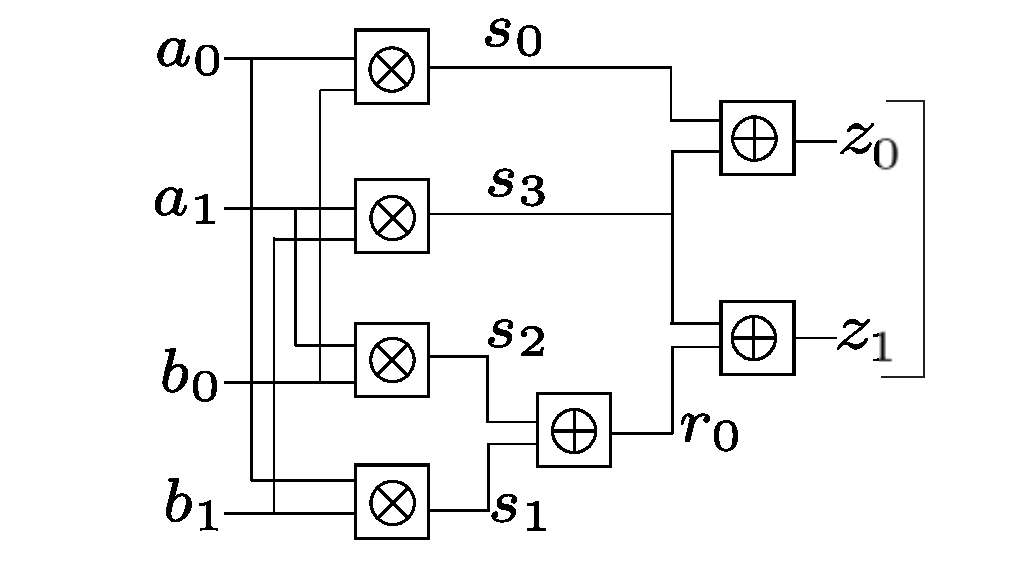
\includegraphics[scale=0.35]{2bitmult.eps}
%}
%\caption{\small A 2-bit Multiplier over ${\mathbb{F}}_{2^2}$. The gate
%  $\otimes$ corresponds to AND-gate, i.e. bit-level multiplication
%  modulo 2. The gate $\oplus$ corresponds to XOR-gate, i.e. addition
%  modulo 2.} 
%\label{fig:mul2bit2}
%\end{figure}
As before, we can describe the functionality of this circuit, $J$, using the
following polynomials: $f_1: Z+z_0+z_1\alpha; ~~f_2: B+b_0+b_1\alpha; ~~f_3: A+a_0+a_1 \alpha
; ~~f_4: s_0+a_0 \cdot b_0; ~~f_5: s_1+a_0 \cdot b_1; ~~f_6:
s_2+a_1 \cdot b_0; ~~f_7: s_3+a_1 \cdot b_1; ~~f_8: r_0+s_1 + s_2;
~~f_9: z_0+s_0 + s_3; ~~f_{10}: z_1 + r_0 + s_3$.
By imposing the monomial order $>_1$, $J+J_0$ is already a Gr\"obner basis, 
where $J_0$ is the ideal of vanishing polynomials of the circuit:
$~~f_{11}: a_0^2+a_0; ~~f_{12}: a_1^2+a_1; ~~f_{13}: b_0^2+b_0;
~~f_{14}: b_1^2+b_1; ~~f_{15}: s_0^2+s_0; ~~f_{16}: s_1^2+s_1;
~~f_{17}: s_2^2+s_2; ~~f_{18}: s_3^2+s_3; ~~f_{19}: r_0^2+r_0;
~~f_{20}: z_0^2+z_0; ~~f_{21}: z_1^2+z_1$. We denote this Gr\"obner
basis as $G_1 = \{f_1, \dots, f_{21}\}$. Using the FGLM algorithm 
("fglm" command in  Singular) we convert $G_1$
from ordering $>_1$ to $G$ with the abstraction term ordering $>$. 
The resulting Gr\"obner basis $G$ contains the 
polynomial $Z \cdot (\alpha+1)+A \cdot B \cdot (\alpha+1)$, 
which can be equivalently reduced to $Z+A \cdot B$.
}
\end{Example}

FGLM exploits concepts from algebraic geometry and sparse linear
algebra to transform the Gr\"obner basis. While a detailed exposition
of FGLM is beyond the scope of this paper, we demonstrate its
operation on the 2-bit multiplier shown in Example
\ref{ex:myapproach}.  

\begin{Example}
\label{ex:approach}
{\it
FGLM begins by taking the least variable in the the abstraction term 
ordering, ($A$ in our case). Starting with $m=0$, it computes $A^m
\xrightarrow{G_1}_+r$. It checks whether the remainder $r$ can be
represented as a linear combination of any remainders calculated thus
far. If so, it adds this  representation to $G$ and moves on to the
next monomial; otherwise it  increments $m$ and repeats $A^m
\xrightarrow{G_1}_+r$ computation. 

\begin{itemize}
\item $A^0 \xrightarrow{G_1}_+ 1$
\item $A^1 \xrightarrow{G_1}_+ a_0+ a_1 \alpha$
\item $A^2 \xrightarrow{G_1}_+ a_0+a_1 \cdot (\alpha+1) $
\item $A^3 \xrightarrow{G_1}_+ a_0 \cdot a_1+a_0+a_1$
\item $A^4 \xrightarrow{G_1}_+ a_0+ a_1 \alpha = A$
\end{itemize}

$A^4$ can be composed of $A$, so $A^4 - A$ is added to $G$. Similarly,
$B^4 - B$ is also added to $G$. Continue to the next variable $Z$ in
the order as we have ``circuit variables'' $> Z > A > B$. 
\begin{itemize}
\item $Z^1 \xrightarrow{G_1}_+ a_0 \cdot b_0+(\alpha) \cdot a_0 \cdot
  b_1+(\alpha) \cdot a_1 \cdot b_0+(\alpha^2) \cdot a_1 \cdot b_1 = 
a_0(b_0 + b_1 \alpha) + a_1\alpha (b_0 + b_1 \alpha) = (a_0 + a_1
\alpha)(b_0 + b_1 \alpha) = A   \cdot B$ 
\end{itemize}
$Z$ is found to be a function of $A$ and $B$, therefore $Z - AB$ is
added to $G$.
}
\end{Example}

FGLM continues to convert the rest of the monomials into the new ordering. However, 
since we are only looking for $Y=\F(A)$ polynomial representation, we
can make this approach even more efficient by restricting the
conversion to only the word-level variables of the circuit. This idea
is currently under development. 

\section{Conclusions}
\label{sec:concl}

This paper has described an approach to derive a word-level, canonical
polynomial representation from combinational circuits using Gr\"obner
bases. Our approach interprets the function of the circuit $f: \B^k
\rightarrow \B^k$ as a polynomial function over Galois fields $f: \Fkk
\rightarrow \Fkk$. By deriving a set of polynomials corresponding to
the circuit (ideal $J + J_0$), and computing its Gr\"obner basis
w.r.t. a specific elimination (abstraction) term order, the canonical
representation of this circuit can be derived. As Gr\"obner basis
computation exhibits high complexity, we are currently investigating
the use of the FGLM algorithm to make our approach scalable. 

% THIS IS SIGPROC-SP.TEX - VERSION 3.1
% WORKS WITH V3.2SP OF ACM_PROC_ARTICLE-SP.CLS
% APRIL 2009
%
% It is an example file showing how to use the 'acm_proc_article-sp.cls' V3.2SP
% LaTeX2e document class file for Conference Proceedings submissions.
% ----------------------------------------------------------------------------------------------------------------
% This .tex file (and associated .cls V3.2SP) *DOES NOT* produce:
%       1) The Permission Statement
%       2) The Conference (location) Info information
%       3) The Copyright Line with ACM data
%       4) Page numbering
% ---------------------------------------------------------------------------------------------------------------
% It is an example which *does* use the .bib file (from which the .bbl file
% is produced).
% REMEMBER HOWEVER: After having produced the .bbl file,
% and prior to final submission,
% you need to 'insert'  your .bbl file into your source .tex file so as to provide
% ONE 'self-contained' source file.
%
% Questions regarding SIGS should be sent to
% Adrienne Griscti ---> griscti@acm.org
%
% Questions/suggestions regarding the guidelines, .tex and .cls files, etc. to
% Gerald Murray ---> murray@hq.acm.org
%
% For tracking purposes - this is V3.1SP - APRIL 2009

\documentclass{acm_proc_article-sp}

%packages
\usepackage[linesnumbered, ruled]{algorithm2e}
\RequirePackage{amssymb, mathptm}
\usepackage{amsbsy}
\usepackage{graphicx}
\usepackage{helvet}
\usepackage{enumerate}
\usepackage{amsmath}
\usepackage{cases}
\usepackage{amsfonts}
\usepackage{graphicx}
\usepackage{multirow}
\usepackage{subfig}
\usepackage{comment}

%new format
\newtheorem{Algorithm}{Algorithm}
\newdef{Definition}{Definition}
\newtheorem{Theorem}{Theorem}
\newtheorem{Lemma}{Lemma}
\newdef{Example}{Example}

\begin{document}

\title{Verification of Sequential Galois Field Circuits using Algebraic Geometry
\titlenote{Version 0.3, refined theory part with normal basis, proposed details for designing 2 examples.}}
%\subtitle{[Extended Abstract]
%\titlenote{A full version of this paper is available as
%\textit{Author's Guide to Preparing ACM SIG Proceedings Using
%\LaTeX$2_\epsilon$\ and BibTeX} at
%\texttt{www.acm.org/eaddress.htm}}}
%
% You need the command \numberofauthors to handle the 'placement
% and alignment' of the authors beneath the title.
%
% For aesthetic reasons, we recommend 'three authors at a time'
% i.e. three 'name/affiliation blocks' be placed beneath the title.
%
% NOTE: You are NOT restricted in how many 'rows' of
% "name/affiliations" may appear. We just ask that you restrict
% the number of 'columns' to three.
%
% Because of the available 'opening page real-estate'
% we ask you to refrain from putting more than six authors
% (two rows with three columns) beneath the article title.
% More than six makes the first-page appear very cluttered indeed.
%
% Use the \alignauthor commands to handle the names
% and affiliations for an 'aesthetic maximum' of six authors.
% Add names, affiliations, addresses for
% the seventh etc. author(s) as the argument for the
% \additionalauthors command.
% These 'additional authors' will be output/set for you
% without further effort on your part as the last section in
% the body of your article BEFORE References or any Appendices.

\numberofauthors{2} %  in this sample file, there are a *total*
% of EIGHT authors. SIX appear on the 'first-page' (for formatting
% reasons) and the remaining two appear in the \additionalauthors section.
%
\author{
% You can go ahead and credit any number of authors here,
% e.g. one 'row of three' or two rows (consisting of one row of three
% and a second row of one, two or three).
%
% The command \alignauthor (no curly braces needed) should
% precede each author name, affiliation/snail-mail address and
% e-mail address. Additionally, tag each line of
% affiliation/address with \affaddr, and tag the
% e-mail address with \email.
%
% 1st. author
\alignauthor
Xiaojun Sun\\
       \affaddr{University of Utah}\\
       \affaddr{Department of Electrical \& Computer Engineering}\\
       \affaddr{Salt Lake City, USA}\\
       \email{xiaojun.sun@utah.edu}
% 2nd. author
\alignauthor
Priyank Kalla\\
       \affaddr{University of Utah}\\
       \affaddr{Department of Electrical \& Computer Engineering}\\
       \affaddr{Salt Lake City, USA}\\
       \email{kalla@ece.utah.edu}
% 3rd. author
%\alignauthor Lars Th{\o}rv{\"a}ld\titlenote{This author is the
%one who did all the really hard work.}\\
%       \affaddr{The Th{\o}rv{\"a}ld Group}\\
%       \affaddr{1 Th{\o}rv{\"a}ld Circle}\\
%       \affaddr{Hekla, Iceland}\\
%       \email{larst@affiliation.org}
%\and  % use '\and' if you need 'another row' of author names
% 4th. author
%\alignauthor Lawrence P. Leipuner\\
%       \affaddr{Brookhaven Laboratories}\\
%       \affaddr{Brookhaven National Lab}\\
%       \affaddr{P.O. Box 5000}\\
%       \email{lleipuner@researchlabs.org}
% 5th. author
%\alignauthor Sean Fogarty\\
%       \affaddr{NASA Ames Research Center}\\
%       \affaddr{Moffett Field}\\
%       \affaddr{California 94035}\\
%       \email{fogartys@amesres.org}
% 6th. author
%\alignauthor Charles Palmer\\
%       \affaddr{Palmer Research Laboratories}\\
%      \affaddr{8600 Datapoint Drive}\\
%%      \affaddr{San Antonio, Texas 78229}\\
%       \email{cpalmer@prl.com}
}
% There's nothing stopping you putting the seventh, eighth, etc.
% author on the opening page (as the 'third row') but we ask,
% for aesthetic reasons that you place these 'additional authors'
% in the \additional authors block, viz.
%\additionalauthors{Additional authors: John Smith (The Th{\o}rv{\"a}ld Group,
%email: {\texttt{jsmith@affiliation.org}}) and Julius P.~Kumquat
%(The Kumquat Consortium, email: {\texttt{jpkumquat@consortium.net}}).}
\date{21 Jan 2014}
% Just remember to make sure that the TOTAL number of authors
% is the number that will appear on the first page PLUS the
% number that will appear in the \additionalauthors section.

\maketitle
\begin{abstract}
Circuits working in Galois fields are increasingly employed in designs like arithmetic component for Elliptic Curve Cryptography (ECC). 
This work proposes a new method to effectively verify sequential circuits in Galois fields. Algebraic geometry
is introduced to describe circuits behavior and expand the definition of implicit state space traversal. Moreover, Gr\"obner basis
representation is adopted for word-level abstraction on circuit variables to address state explosion problem
with BDDs. Experiments are run with fast Gr\"obner basis computation engine to get competitive results.
\end{abstract}

% A category with the (minimum) three required fields
\category{EDA5.1}{Verification}{Functional, transaction-level, RTL, and gate-level modeling and verification of hardware design}
%A category including the fourth, optional field follows...
%\category{D.2.8}{Software Engineering}{Metrics}[complexity measures, performance measures]

\terms{Verification, Algorithms}

\keywords{Verification, Sequential, Galois Fields, Algebraic Geometry} % NOT required for Proceedings

\section{Essential Theory}
\subsection{Polynomial Representation}
A typical sequential circuit is composed as figure \ref{fig:sequential}. The combinational logic has primary input $x$, state
inputs $\{s_0, s_1, \dots, s_{k-1}\}$, primary output $z$ and state outputs $t_0, t_1, \dots, t_{k-1}$. State outputs
are latched into registers, which will be fed back to state inputs in next clock cycle.

\begin{figure}
\centering
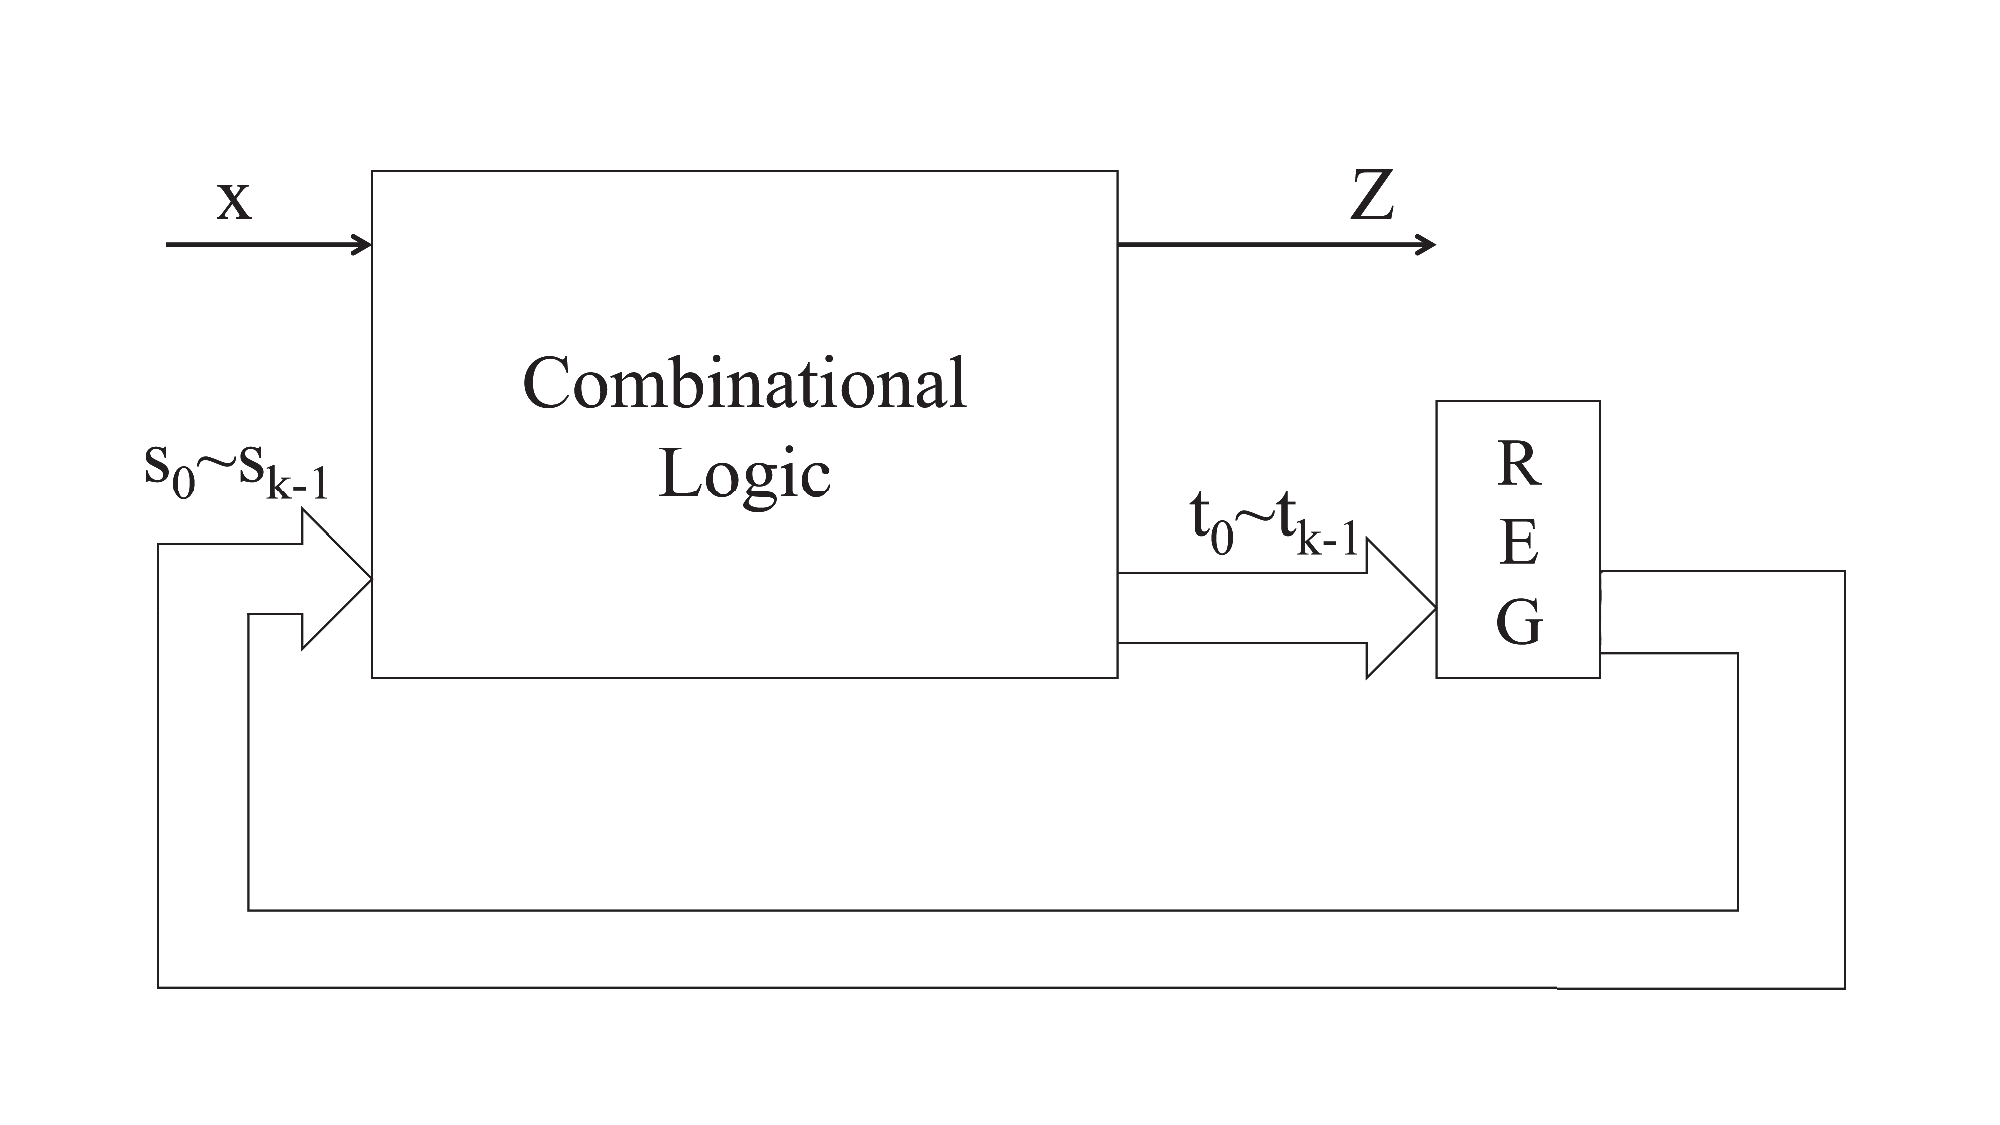
\psfig{file=./sequential_fig.ps, height=2in, width=3.5in,}
\caption{A typical sequential circuit block view}
\label{fig:sequential}
\end{figure}

A transition function $\Delta$ is a Boolean function about state outputs and all inputs, i.e.
\begin{displaymath}
t_i = \Delta_i(x, s_0, s_1, \dots, s_{k-1})
\end{displaymath}
This constrain could also be written in the form of equation $polynomial = 0$:
\begin{displaymath}
t_i - \Delta_i(x, s_0, s_1, \dots, s_{k-1}) = 0
\end{displaymath}
Solution to this equation is limited within $\{0, 1\}$, which is set of all elements in Galois field $\mathbb{F}_2$.
Furthermore, there exists a one-to-one corresponding relation from Boolean space to Galois field on higher dimension: 
$\mathbb{B}^k \to \mathbb{F}_{2^k}$, which means it is possible to find a set of elements in $\mathbb{F}_{2^k}$ representing
all Boolean values every bit of a bit vector can take. In Galois field, a as \ref{table:booltogalois} shows.
\begin{table}[h]
\centering
\caption{Bit-vector, Exponential and Polynomial representation of
elements in  ${\mathbb{F}}_{2^4} = {\mathbb{F}}_2[x]
\pmod{x^4+x^3+1}$}\label{table:booltogalois}  
\begin{tabular}{|c|c||c|c|} 
\hline
$a_3a_2a_1a_0$ & Polynomial     &$a_3a_2a_1a_0$ & Polynomial  \\
\hline
$0000$        & $0$           & $1000$  &$\alpha^3$\\
\hline
$0001$        & $1$           & $1001$  & $\alpha^3 + 1$\\
\hline
$0010$        &  $\alpha$       & $1010$ & $\alpha^3 + \alpha$  \\
\hline
$0011$        &  $\alpha + 1$   & $1011$ &  $\alpha^3+\alpha+1$\\
\hline
$0100$        &  $\alpha^2$     &  $1100$ &  $\alpha^3 + \alpha^2$\\
\hline
$0101$        & $\alpha^2 + 1$ & $1101$  & $\alpha^3+\alpha^2+1$\\
\hline
$0110$        &  $\alpha^2 + \alpha$ & $1110$ &  $\alpha^3+\alpha^2+\alpha$\\
\hline
$0111$        & $\alpha^2+\alpha+1$ & $1111$ & $\alpha^3+\alpha^2+\alpha+1$\\
\hline
\end{tabular}
\end{table}
A word-level representation on state inputs/outputs can be attained through above correspondence. If the set of 
state inputs $\{s_0, s_1, \dots, s_{k-1}\}$ is denoted by $S$ taking values from $\mathbb{F}_{2^k}$, and
set of outputs $\{t_0, t_1, \dots, t_{k-1}\}$ is denoted by $T$, a word-level transition function can be written as
\begin{displaymath}
T - \Delta(x, S) = 0
\end{displaymath}
If $T - \Delta(x, S)$ is taken as a polynomial $f$, then $f \in \mathbb{F}_{2^k}[x]\ mod\ P(\alpha)$.
\subsection{Gr\"obner Basis Theory}
Gr\"obner basis is used to calculate desired results out of a set of polynomials.
If there exists multiple polynomials $\{f_1, f_2, \dots, f_r\}$ representing constrains on $T, x$ and $S$,
then all polynomials should simultaneously equal to $0$.
\begin{displaymath}
\left\{
  \begin{array}{lc}
  f_1 & = 0\\
  f_2 & = 0\\
  \dots & \ \\
  f_r & = 0
  \end{array} \right.
\end{displaymath}
Solution to these equations is set of values of $(T, x, S)$, which is called \textbf{Variety} of \textbf{ideal}
$I = \langle f_1, f_2, \dots, f_r\rangle $.

Calculate Reduced Gr\"obner Basis (RGB) from ideal $I$ with \textbf{elimination term order}, there exists a polynomial contains
only $T$, if the values of states input $S$ and primary input $x$ are given in the form of polynomials and included by $I$,
the values of $T$ can be computed.

Otherwise, if RGB calculation is manipulated under \textbf{abstraction term order}, there exists a polynomial in
the form of $T - \mathcal{F}(x, S)$ representing transition function. In next clock cycle, assign new state input $S'$ with $T$, the next
state can be computed again, result is polynomial $T' - \mathcal{F}(x', S')$. 

\subsection{Normal Basis Representation}

Let $\beta$ be an element in the Galois field $F_{2^n}$ constructed by primitive element $\alpha$ and minimal polynomial
$P(\alpha)$. Then a basis in the form $\{\beta, \beta^2, \beta^4, \beta^8, ... ,\beta^{2^{n-1}}\}$ is a
\emph{Normal Basis}; here $\beta$ is called \emph{Normal Element}.

For arithmetic operations in Galois fields, squaring and multiplication (with modulus) can be greatly simplified if 
normal basis representation is adopted to represent operands.
\begin{Example}
\label{ex:nb_sq}
Element squaring: In $F_{2^n}$, all coefficients which can be divided by 2 are reduced, so 
following equality holds for all field elements $a$ and $b$:
$$(a+b)^2 = a^2 + b^2$$ 
Apply this rule on element squaring of standard/polynomial basis:
\begin{align}
& (b_0\beta + b_1\beta^2 + b_2\beta^4 + \dots + b_{n-1}\beta^{2^{n-1}})^2 \nonumber\\
&= b_0^2\beta^2 + b_1^2\beta^4 + b_2^2\beta^8 + \dots + b_{n-1}^2\beta^{2^n} \nonumber\\
&= b_{n-1}^2\beta + b_0\beta^2 + b_1\beta^4 + \dots + b_{n-2}\beta^{2^{n-1}} \nonumber
\end{align}
using Fermat's little theorem $\beta^{2^n} = \beta$. This shows that squaring of field elements
represented by normal bases can be easily completed by operating a simple right-cyclic rotation.
\end{Example}

\begin{Example}
\label{ex:nb_multi}
Normal basis multiplication: There are 2 binary vectors representing operands of multiplication in normal
basis: $$A = (a_0, a_1, \dots, a_{n-1}),\ B = (b_0, b_1, \dots, b_{n-1})$$ 
the product is also written in normal basis representation: $$C = A*B = (c_0, c_1, \dots, c_{n-1})$$
Describe calculation procedure for the most significant digit of product with a function: 
$$c_{n-1} = f(a_0, a_1, \dots, a_{n-1}; b_0, b_1, \dots, b_{n-1})$$
Square both side: $C^2 = A^2*B^2$, i.e. the second significant digit 
$$c_{n-2} = f(a_{n-1}, a_0, a_1, \dots, a_{n-2}; b_{n-1}, b_0, b_1, \dots, b_{n-2})$$ 
By this method it is easy to get all digits of product $C$.
\end{Example}
  
\section{Algebraic Geometry Approach}
\subsection{State Space Traversal}

\begin{figure}
\centering
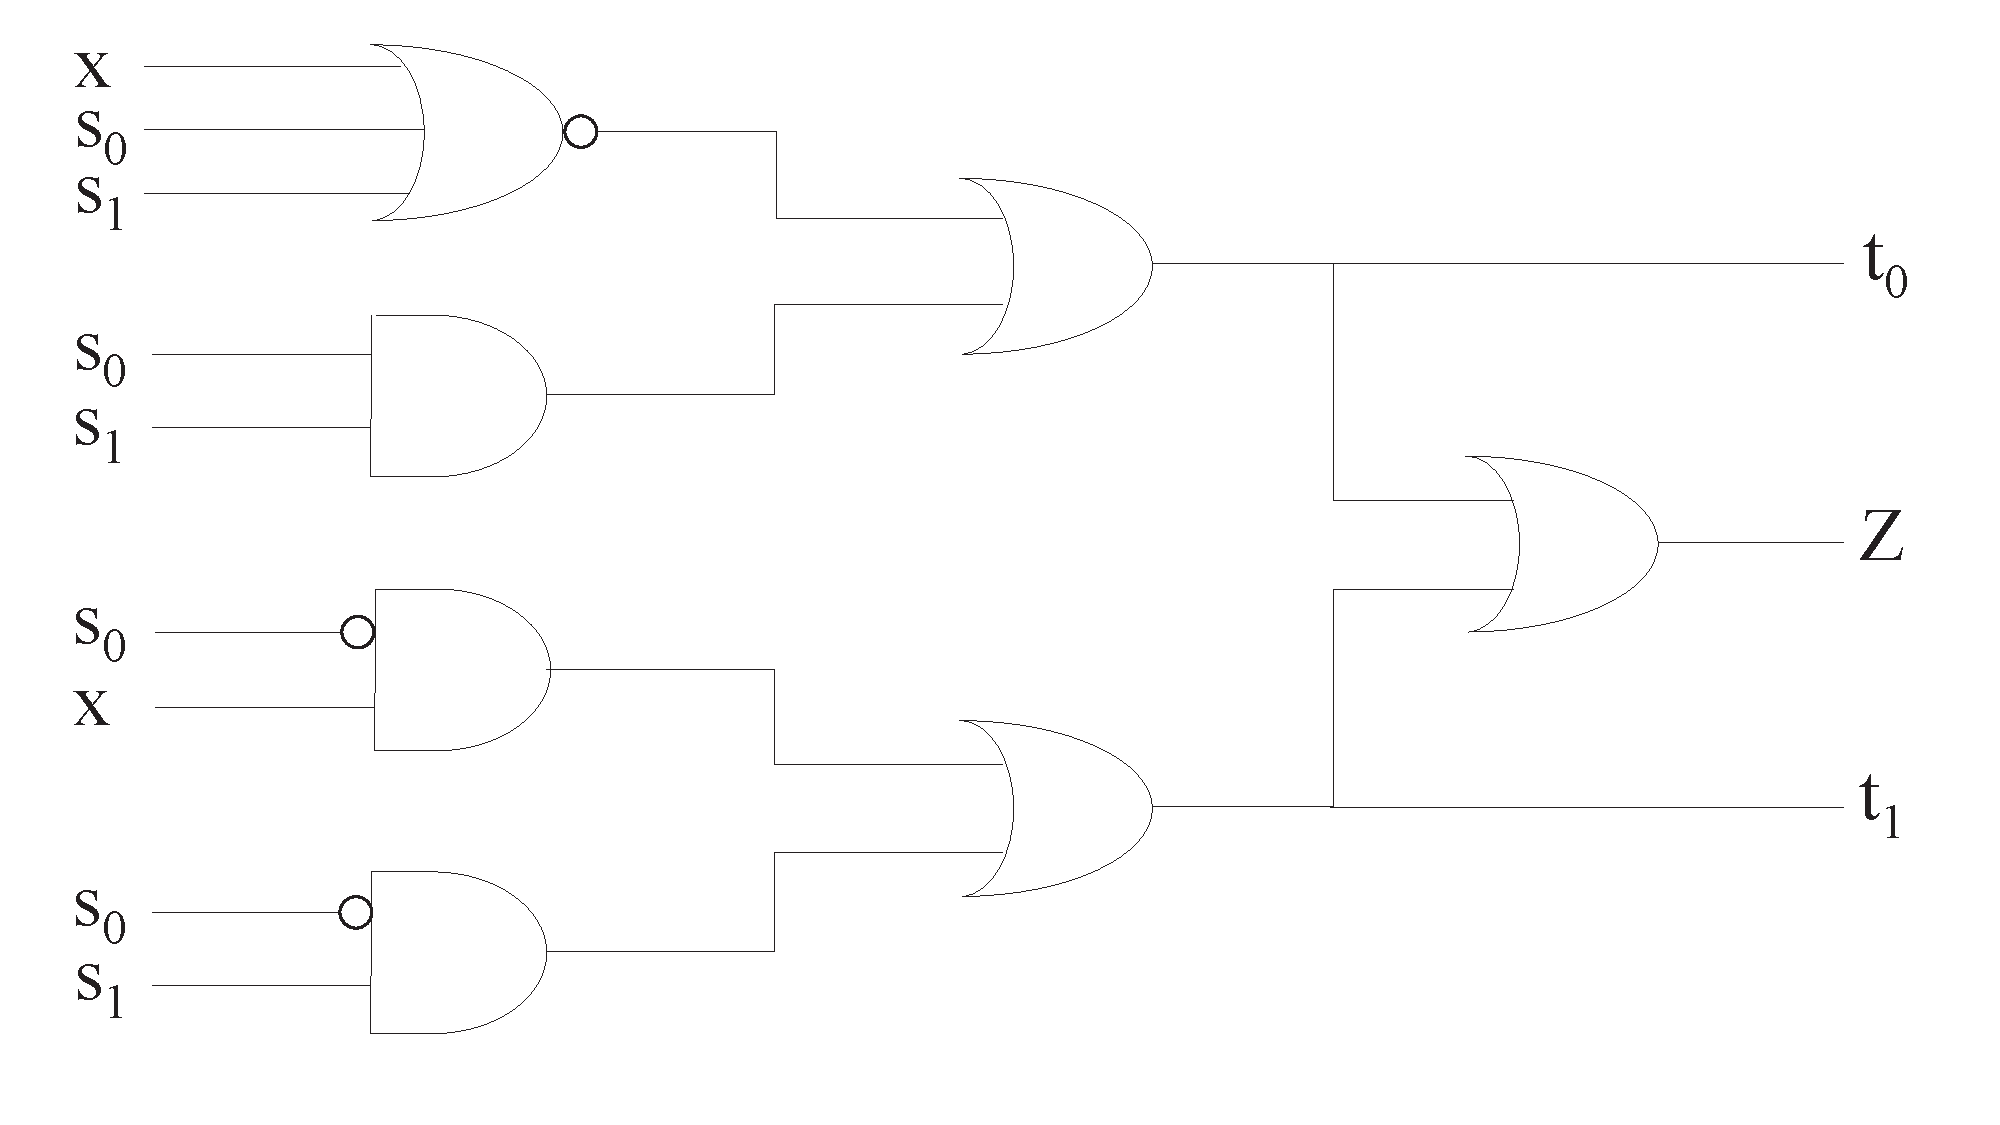
\psfig{file=./fsm_fig.ps, height=2in, width=3.5in,}
\caption{Gate-level circuit of combinational logic block of sample FSM}
\label{fig:fsm}
\end{figure}

\begin{figure}
\centering
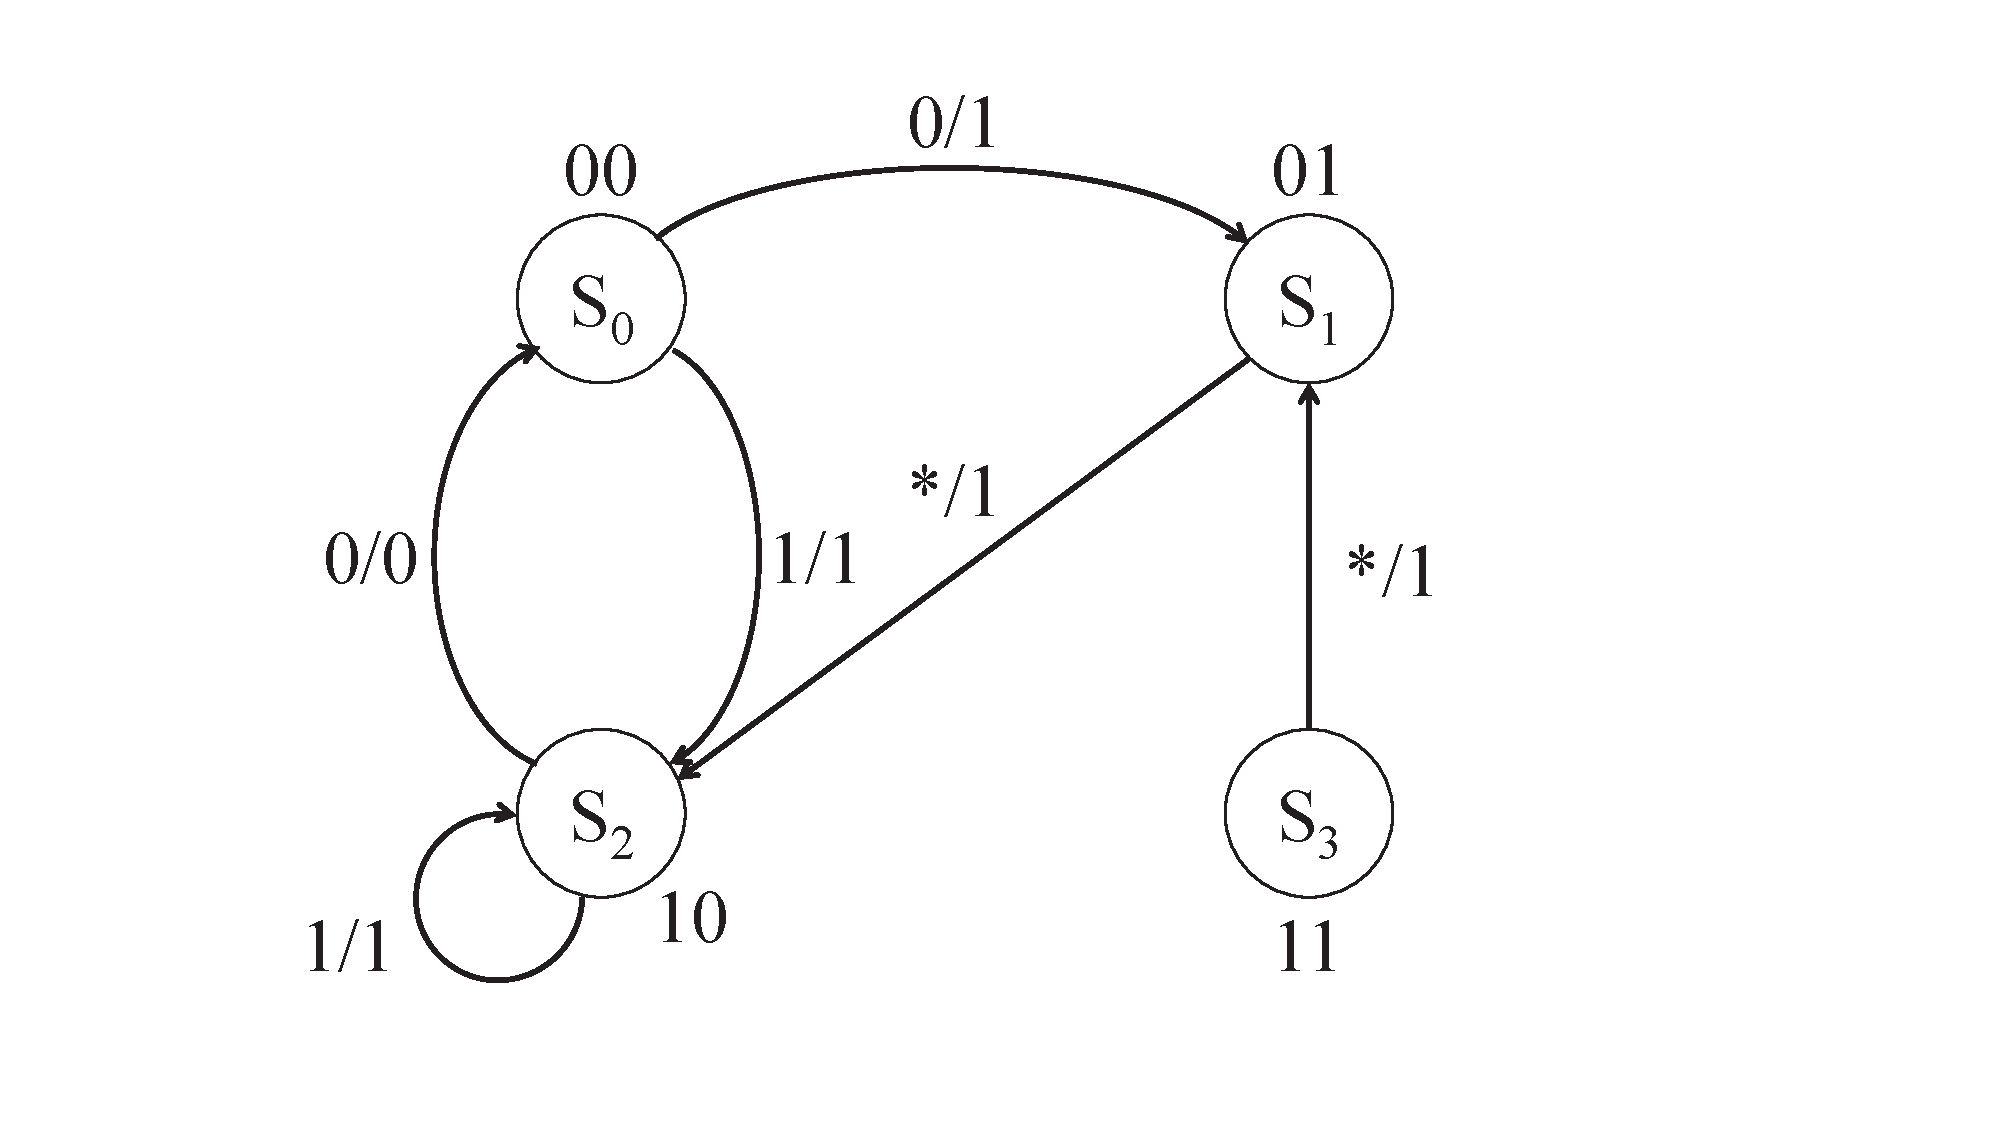
\psfig{file=./stg_fig.ps, height=2in, width=3.5in,}
\caption{State transition graph of sample FSM}
\label{fig:stg}
\end{figure}

The first example is a mealy finite state machine (FSM). Gate-level circuits of combinational logic
is figure \ref{fig:fsm}, $x$ is primary input,
$\{s_0, s_1\}$ are state inputs, $Z$ is primary output and $\{t_0, t_1\}$ are state outputs.
Word-level state input is $S = s_0 + s_1\cdot\alpha$, output is $T = t_0 + t_1\cdot\alpha$. In Galois field
$\mathbb{F}_{2^2}$, bit-level variables $x, s_0, s_1, Z, t_0, t_1$ can take values from $\{0, 1\}$, while
word-level variables $S, T$ may take values from $\{0, 1, \alpha, 1 + \alpha\}$. State transition graph (STG)
showed in figure \ref{fig:stg} uses 2-bit Boolean vector to represent 4 states $\{S_0, S_1, S_2, S_3\}$, which
could be converted to elements in $\mathbb{F}_{2^2}$ similarly as table \ref{table:booltogalois} shows.

One important technique to check sequential equivalence is \textbf{state space traversal}. In this example,
Breath-First-Search (BFS) is employed for traversal, which can be described with following algorithm:

\begin{algorithm}[hbt]
\SetAlgoNoLine
 \KwIn{Transition functions $\Delta$, initial state $S^0$}

  $from^0 = reached = S^0$\;
  \Repeat{$new^i == 0$}
  {
  	$i \gets i + 1$\;
	$to^i \gets$Img$(\Delta, from^{i-1})$\;
	$new^i \gets to^i \cap \overline{reached}$\;
  	$reached \gets reached \cup new^i$\;
	$from^i \gets new^i$\;
  }
\Return{$reached$}
\caption {Breadth-first Traversal Algorithm}\label{alg:BFS}
\end{algorithm}

Our approach is implementing state space traversal by refined BFS algorithm combined with polynomial representation
and Gr\"obner basis theory. In practice, this example will show how to apply concepts and techniques from algebraic
geometry on each line of above BFS algorithm.

\subsection{States and Varieties of Ideal}

\begin{Theorem}
State variables $S, T$ and sets of states such as $from^i, to^i$ can always be represented as varieties of ideals.
\end{Theorem}
For example in Line 1 of BFS algorithm, assume initial state is $S_3$ in figure \ref{fig:stg}, then corresponding
polynomial $f = \mathcal{F}(S^0) = S^0 - 1 - \alpha$. Consider an ideal $I$ with only one generator $f$, its variety
$V(I) = \{\gamma\ |\ \gamma \in \mathbb{F}_{2^2}, \gamma - 1 - \alpha = 0\}$, which equals to $\{1 + \alpha\}$, the only
valid value $S^0$ can take.

If an ideal contains multiple polynomial specifications, it is necessary to compute Gr\"obner basis with elimination term
order to get one polynomial only on desired variable. In first iteration of Line 4, $to^i$ has multiple specifications,
some of them are transition functions on bit-level:
\begin{displaymath}
\begin{array}{ll}
f_1:& t_0 - (\overline{x}\ and\ \overline{s_0}\ and\ \overline{s_1})\ or\ (s_0\ and\ s_1) \\
f_2:& t_1 - (\overline{s_0}\ and\ x)\ or\ (p\ and\ \overline{s_1})\
\end{array}
\end{displaymath}
And some are bits-to-word definitions fitting polynomial representation of elements in $\mathbb{F}_{2^2}$:
\begin{displaymath}
\begin{array}{ll}
f_3:& S - s_0 - s_1\alpha \\
f_4:& T - t_0 - t_1\alpha
\end{array}
\end{displaymath}
And an polynomial about initial state as mentioned above:
\begin{displaymath}
f_5:\  S - 1 - \alpha
\end{displaymath}
And the rests are vanishing polynomials for every variable, bit-level and word level:
$f_6: x^2 - x; f_7: t_0^2 - t_0; f_8: t_1^2 - t_1; f_9: S^4 - S; f_{10}: s_0^2 - s_0;
f_{11}: s_1^2 - s_1; f_{12}: T^4 - T$

Transition equations here contains some Boolean operators, they can be re-written in terms of operations in Galois fields. 
In $\mathbb{F}_{2}$, let $TRUE = 1, FALSE = 0$, for either element $a$ in this field, considering $0 + 0 = 1 + 1 \equiv 0\ (mod\ 2)$
and $0 + 1 = 1 + 0 \equiv 1\ (mod\ 2)$, the inverse of $a$ is: $\overline{a} = 1 + a$. Similarly all Boolean operators
can be converted within $\mathbb{F}_{2}$, table \ref{table:booltogalois_op} gives part of them and their corresponding
operations in $\mathbb{F}_{2}$:
Also note that there is no specification on initial primary input $x$, in Gr\"obner basis approach this means $x$ is smoothed by
reversely using Shannon's expansion.
\begin{table}
\centering
\caption{Some Boolean operators and corresponding operations in $\mathbb{F}_{2}$}
\label{table:booltogalois_op}
\begin{tabular}{|c|c|} \hline
Boolean operator & operation in $\mathbb{F}_{2}$\\ \hline
$\overline{a}$ & $1 + a$\\ \hline
$a\ and\ b$ & $ab$\\ \hline
$a\ or\ b$ & $a + b + ab$\\ \hline
$a \oplus b$ & $a + b$\\
\hline\end{tabular}
\end{table}
Using elimination term order: $others\ >\ bit$-$level\ inputs/outputs\ >\ S\ >\ T$, compute Gr\"obner basis for ideal
$J = \langle f_1, f_2, \dots, f_{12}\rangle $, the result will include one polynomial $f_T$ contains only variable $T$. In this example,
$f_T = T + 1$. This polynomial equals to $T - 1$ since coefficients of polynomial representation in $\mathbb{F}_{2^2}$ are
limited within $\mathbb{F}_{2}$, where $1 \equiv -1\ (mod\ 2)$. Solution to $f_T = 0$ is $T = 1$, which shows that next
state the machine just reached is $\{S_1(01)\}$.

\subsection{Application of Algebraic Geometry}

There are some difficulties with polynomial representation when executing Line 5 and Line 6, it is necessary to explore
how \textbf{Union}, \textbf{Intersection} and \textbf{Complement Set} works in Galois field $\mathbb{F}_{2^k}$. Since
state set variables $from^i, to^i, reached$ all have single polynomial, consider an ideal $I$ with single generator $I = \langle f\rangle $.
Example: assume $I = \langle f\rangle  = \langle T^2 + (1+\alpha)\cdot T+\alpha\rangle $, its variety $V(I) = \{a\ |\ a \in \mathbb{F}_{2^2}\ and\ f(a) = 0\} = \{1, \alpha\}$.
So it is reasonable to specify: union, intersection and complement set mentioned in this paper are all functions on \textbf{varieties}.
To better discuss this problem, introduce following concepts from algebraic geometry:
\begin{Definition}
\label{def:sum}
({\bf Sum of Ideals}) If $I$ and $J$ are ideals in $k[x_1, \dots, x_n]$, then the 
{\bf sum} of $I$ and $J$, denoted by $I + J$, is the set
  \begin{equation}
  I + J = \{f + g\ |\ f \in I \ and\  g \in J\}.
  \end{equation}
Furthermore, if $I = \langle f_1, \dots, f_r\rangle$ and 
$J = \langle g_1, \dots, g_s\rangle$, then 
$I + J = \langle f_1, \dots, f_r, g_1, \dots, g_s\rangle$.
\end{Definition}
\begin{Definition}
\label{def:prod}
({\bf Product of Ideals}) If $I$ and $J$ are ideals in $k[x_1, \dots, x_n]$, then the
{\bf product} of $I$ and $J$, denoted by $I \cdot J$, is defined to be the ideal generated 
by all polynomials $f \cdot g$ where $f \in I$ and $g \in J$. Furthermore, let
$I = \langle f_1, \dots, f_r\rangle$ and $J = \langle g_1, \dots, g_s\rangle$, then
  \begin{equation}
  I \cdot J = \langle f_ig_j\ |\ 1 \leq i \leq r, 1 \leq j \leq s\rangle .
  \end{equation}
\end{Definition}
\begin{Definition}
({\bf Quotient of Ideals}) If $I$ and $J$ are ideals in $k[x_1, \dots, x_n]$, then $I:J$
is the set
  \begin{equation}
  \{f \in k[x_1, \dots, x_n]\ |\ f\cdot g \in I, \forall g \in J\}
  \end{equation}
and is called the {\bf ideal quotient} of $I$ by $J$.
\end{Definition}
These concepts can lead the way to solution by adopting following theorems:
\begin{Theorem}
\label{thm:unionintersect}
If $I$ and $J$ are ideals in $k[x_1, \dots, x_n]$, then ${\bf V}(I + J) = {\bf V}(I)
\bigcap {\bf V}(J)$ and ${\bf V}(I \cdot J) = {\bf V}(I) \bigcup {\bf V}(J)$.
\end{Theorem}
\begin{Theorem}
\label{thm:quotient}
If $I, J$ are ideals with only one generator, then ${\bf V}(I:J) ={\bf V}(I) - {\bf V}(J)$.
\end{Theorem}
Proof to these theorems are referred to (that yellow book?) and (my write-up?).

For varieties intersection $\{1\}\bigcap\{1, \alpha\}$, calculate ideal sum $\langle T+1, T^2 + (1+\alpha)\cdot T+\alpha\rangle  = \langle T+1\rangle $,
its variety is $\{1\}$; for varieties union $\{1,1+\alpha\}\bigcup\{1+\alpha\}$, calculate
ideal product $\langle (T+1+\alpha)\cdot(T^2 + (1+\alpha)\cdot T+\alpha)\rangle  = \langle T^3 + 1\rangle $, its variety
is $\{1, \alpha, 1+\alpha\}$; for complement set of variety $\{1, \alpha\}$, the universal set is
the variety of ideal of vanishing polynomial $V(\langle T^4-T\rangle ) = \{0,1,\alpha,1+\alpha\}$,
so $\overline{V(\langle T^2 + (1+\alpha)\cdot T+\alpha\rangle )} = V(\langle T^4-T\rangle ) - V(\langle T^2 + (1+\alpha)\cdot T+\alpha\rangle )$,
which equals to $V(\langle T^4-T\rangle :\langle T^2 + (1+\alpha)\cdot T+\alpha\rangle ) = V(\langle T^2+(1+\alpha)\cdot T\rangle )$,
the result is $\{0,1+\alpha\}$.

From discussion above, the BFS traversal is completely implemented in Galois field.
If the initial input is $S_3$: $S + 1 + \alpha$, the final return value will be set of
reachable states: $T^4 + T$, i.e. the universal set, $\{S_0, S_1, S_2, S_3\}$.

\subsection{Discussion on Ideal quotient and its generator}
In nature, we are looking varieties as the solutions to specific polynomial $f=0$ WITHIN $\mathbb{F}_{2^n}$, because (affine) varieties are defined
within algebraic closure $k^n$ but we only care about those fall in $\mathbb{F}_{2^n}$.

Theorem \ref{thm:unionintersect} related to DEF. \ref{def:sum} and \ref{def:prod} counts on ideal generators, so there will be no ambiguity on 
new ideals we get from this theorem. It also appeared in Avrunin's CAV paper. The only problem is what ideal quotient operation will give us.
This should be further discussed because the completeness of our algebraic geometry approach will benefit from it. \emph{Singular} has the function of
ideal quotient, so ask from the author maybe another choice.

If we put this conception aside, it is also feasible to define complement set from "solution to 
equation" sense. Assume $f(x) = x + 1 + \alpha = 0$, its solution within $\mathbb{F}_{2^2}$ 
is $\{1+\alpha\}$; meanwhile solutions to vanishing polynomial $v(x) = x^2 + x = 0$ are
$\{0,1,\alpha,1+\alpha\}$. Now compute solutions to $$g(x) = \frac{v(x)}{f(x)} = 0$$,
this requires $v(x) = 0$ and $f(x) \neq 0$, which means the complement set of solution 
to $f(x) = 0$.

Issues to this interpretation: (a) Is $v(x)$ always divisible by $f(x)$? (b) Is $v(x)=0$ and
$f(x) \neq 0$ equivalent with $g(x)=0$ on their solutions? Could $f(x)$ equal to $0$?

\section{Functional Verification}
\subsection{Sequential Galois Arithmetic Multiplier}
Our experiment is to verify the function of a Galois field multiplier after certain clock cycles.
The following design is Sequential Multiplier with Parallel Output (SMPO),
a Normal Basis multiplier based on Massey-Omura algorithm. Inputs and outputs
are all 5-bit word taking value from ${\mathbb F}_{2^5}$. After loading operands
 A and B, setting all output latches to 0 and running for 5 iterations, the 
output should be $R = A\cdot B$ (mod $x^5 + x^2 + 1$).
\begin{figure}
\centering
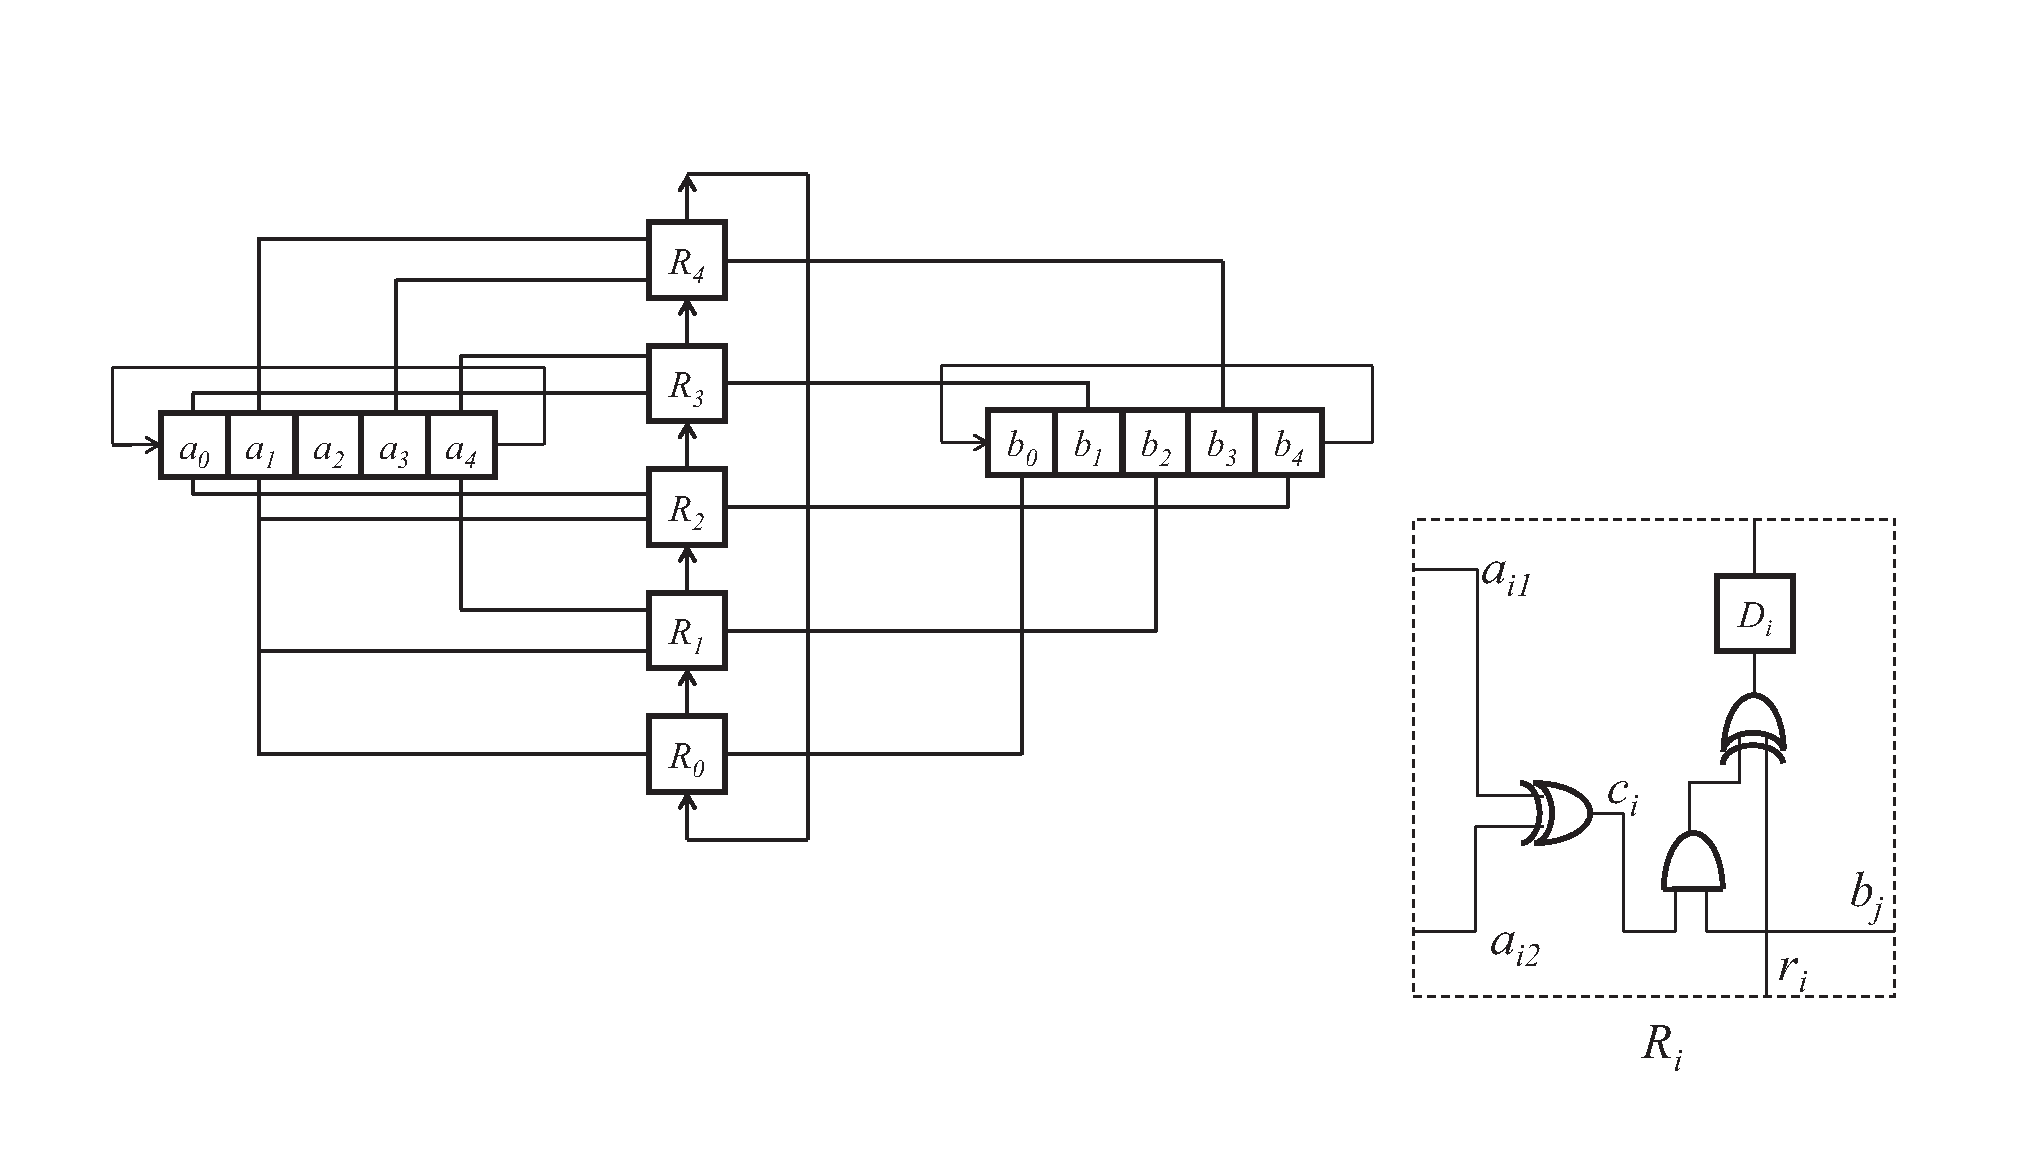
\epsfig{file=./mySMPO.eps, height=2in, width=3.5in}
\caption{5-bit SMPO}
\label{fig:SMPO}
\end{figure}
Similarly, build elimination ideal for all gates/operations and induce
initial states of latches. However, instead of eliminating all variables
to one, this example adopts abstraction term order
and keeps the polynomial contains function between output and inputs.
Here the lex ordering is $\{others\} > R > \{A, B\}$, and objective
polynomial is $R + \mathcal{F}(A, B)$.

Apply this approach to calculate image in BFS traversal, but modify algorithm
\ref{alg:BFS} to make it adapt 5 steps reachable states enumeration.
The result is $R + AB$, which validates the function of this circuit.

\subsection{Gr\"obner basis based Approach}

For 5-bit normal basis multiplication, the $i$-th digit of product can be written as
\begin{align}
R_i &= b_ia_{i+1} + b_{i+1}(a_i + a_{i+3}) + b_{i+2}(a_{i+3} + a_{i+4}) \nonumber\\
&+ b_{i+3}(a_{i+1} + a_{i+2}) + b_{i+4}
(a_{i+2} + a_{i+4}),\ 0\leq i\leq 4 \nonumber
\end{align}
It is possible to calculate every conjunctive term in the product simultaneously within one clock cycle,
on distinct bits. 
Use cyclic similarity of above function, following executions are operated: 
\begin{Example}
Sequential Multiplier Protocol:
\begin{itemize}
\item \textbf{Initial}\ \ $R_0 = R_1 = R_2 = R_3 = R_4 = 0$
\item \textbf{Clock 1}\ \ $R_0 = a_1b_0, R_1 = b_2(a_1 + a_4), R_2 = b_4(a_0 + a_1), R_3 = b_1(a_4 + a_0), 
			R_4 = b_3(a_1 + a_3)$
\item \textbf{Clock 2}\ \ $R_0 = b_3(a_1 + a_3) + a_0b_4, R_1 = a_1b_0 + b_1(a_0 + a_3), R_2 = b_2(a_1 + a_4)
			+ b_3(a_4 + a_0), R_3 = b_4(a_0 + a_1) + b_0(a_3 + a_4), R_4 = b_1(a_4 + a_0) + b_2(a_0 + a_2)$
\item \textbf{$\dots$}
\item \textbf{Clock 5}\ \ $R_0 = c_0, R_1 = c_1, R_2 = c_2, R_3 = c_3, R_4 = c_4$, i.e. $R = A\cdot B$.
\end{itemize}
\end{Example}

In BFS algorithm, the \textbf{Image} function is implemented by constructing an elimination ideal then 
compute its Gr\"obner basis. 
\begin{Example}
\label{ex:SMPO}
For 5-bit SMPO, the ideal consists of (for the first clock cycle):

(a) {\bf Gate descriptions:}
$a_1+a_4+c_1, a_1+a_0+c_2, a_0+a_4+c_3, a_1+a_3+c_4,
		  a_1b_0+r_4+R_0, c_1b_2+r_0+R_1, c_2b_4+r_1+R_2, c_3b_1+r_2+R_3, c_4b_3+r_3+R_4;$
		  
(b) {\bf Word-level variables:}
$A+a_0\alpha^5+a_1\alpha^{10}+a_2\alpha^{20}+a_3\alpha^9+a_4\alpha^{18},
		  B+b_0\alpha^5+b_1\alpha^{10}+b_2\alpha^{20}+b_3\alpha^9+b_4\alpha^{18},
		  r+r_0\alpha^5+r_1\alpha^{10}+r_2\alpha^{20}+r_3\alpha^9+r_4\alpha^{18},
		  R+R_0\alpha^5+R_1\alpha^{10}+R_2\alpha^{20}+R_3\alpha^9+R_4\alpha^{18};$
		  
(c) {\bf Vanishing polynomials:}
		 $ a_0^2+a_0, a_1^2+a_1, a_2^2+a_2, a_3^2+a_3, a_4^2+a_4,
		  b_0^2+b_0, b_1^2+b_1, b_2^2+b_2, b_3^2+b_3, b_4^2+b_4,
		  r_0^2+r_0, r_1^2+r_1, r_2^2+r_2, r_3^2+r_3, r_4^2+r_4,
		  R_0^2+R_0, R_1^2+R_1, R_2^2+R_2, R_3^2+R_3, R_4^2+R_4,
		  c_1^2+c_1, c_2^2+c_2, c_3^2+c_3, c_4^2+c_4,
		  A^{32}+A, B^{32}+B, r^{32}+r, R^{32}+R;$
		  
(d)	{\bf Feedback input:}	  $r_{in}$.

Polynomial $r_{in}$ equals to $from^{i-1}$ in Line 4, BFS algorithm. Under abstraction term ordering,
polynomial $to^i$ is assigned with a polynomial in result Gr\"obner basis which has the form $R + \mathcal{F}(A,B)$. 
Since all outputs are connected to feedback inputs
in SMPO, Line 5 and 6 will be neglected. Line 7 is finished by replace current output $R$ with previous 
output $r$. Initially $r_{in} = 0$.

In next clock cycle, $r_{in} = r + \mathcal{F}(A,B)$ updated from latest result; simultaneously operands
$A$ and $B$ have been cyclically shifted, so gate descriptions in (a) should be modified accordingly. The 
loop is operated for 5 times, result from the last step's Gr\"obner basis should be polynomial $R + AB$.
\end{Example}

This experiment can be repeated on $n$-bits SMPO after running for $n$ clock cycles.

\section{Fast Gr\"obner basis computation}
\subsection{Refined abstraction term order (RATO)}
A lexicographic order constrained by following relation $>_{r}$: "circuit variables ordered reverse topologically" $>$ 
"designated word-level output" $>$ "word-level inputs" is called the \emph{Refined Abstraction Term Order (RATO)}.

In Buchberger's algorithm, the specification polynomial (Spoly) for each pair is calculated. In RATO, most polynomials
have relatively prime leading terms/monomials (which means $Spoly \xrightarrow{J+J_0}_{+} 0$) except one pair:
word-level polynomial corresponding to outputs and its leading bit-level variable's gate description polynomial.
Its remainder $r$ lets following lemma hold:

\begin{Lemma}
\label{lem:1}
$r$ will only contain primary inputs (bit-level and word-level) and word-level output; furthermore, there will be one and
only one term containing word-level output whose monomial is word-level output itself rather than higher order form.
\end{Lemma}

\begin{proof}
First proposition is easy to prove by contradiction. Second part, the candidate pair of polynomials only have one term of
single word-level output variable (say it is $R$) and this term is the last term under RATO, which means there is only one term with
$R$ in Spoly. Meanwhile in other polynomials from $J+J_0$ there is no such term containing $R$, so this term will be
kept to remainder $r$, in first degree.
\end{proof}

\begin{Example}
The elimination ideal for 5-bit SMPO (Ex.\ref{ex:SMPO}) could be rewritten under RATO:
\begin{align}
&(R_0,R_1,R_2,R_3,R_4)>(r_0,r_1,r_2,r_3,r_4)\nonumber\\&>(c_1,c_2,c_3,c_4,b_0,b_1,b_2,b_3,b_4)\nonumber\\
&>(a_0,a_1,a_2,a_3,a_4)>R>r>(A,B)\nonumber
\end{align}
Thus the candidate pair is
$(f_w,f_g), f_w = R_0+r_4+b_0\cdot a_1, f_g =R_0\alpha^5+R_1\alpha^{10}+R_2\alpha^{20}+R_3\alpha^9+R_4\alpha^{18} + R$.
Result after reduction is:
\begin{align}
&Spoly(f_w,f_g) \xrightarrow{J+J_0}_{+}\nonumber\\
&r_1+(\alpha)r_2+(\alpha^4+\alpha^2)r_3+(\alpha^3+\alpha^2)r_4+(\alpha^3)b_1a_1+(\alpha^4+\alpha^2)b_1a_2\nonumber\\
+&(\alpha^3+\alpha+1)b_1a_3+(\alpha^3+\alpha)b_1a_4+(\alpha+1)b_1A+(\alpha^4+\alpha^2+\alpha)b_2a_1\nonumber\\
+&(\alpha^4+\alpha^3+\alpha^2+\alpha)b_2a_4+(\alpha^3+\alpha^2+1)b_3a_1+(\alpha)b_3a_3\nonumber\\
+&(\alpha^2+\alpha+1)b_4a_1+(\alpha+1)b_4a_2+(\alpha^4+\alpha^2)b_4a_3+(\alpha^4+\alpha^3+\alpha+1)b_4a_4\nonumber\\
+&(\alpha^3+1)b_4A+(\alpha^4+\alpha^3+\alpha^2+1)a_1B+(\alpha^4+\alpha^3+\alpha^2+1)R\nonumber
\end{align}
The remainder satisfies Lemma \ref{lem:1}.
\end{Example}

\subsection{Bit-level Variable Substitution (BLVS)}
The remainder from \emph{Spoly} contains some bit-level variables, and our objective is to get a polynomial contains only word-level variables
(such as $R+\mathcal{F}(A,B)$). One possible method is to rewrite bit-level variables in term of function on word-level
variables, i.e. $a_i = \mathcal{G}(A)$, then do substitution. A Gaussian-elimination-fashion approach could be applied to
compute corresponding $\mathcal{G}(A)$ efficiently.

\begin{Example}
{\bf Objective}:\ Abstract polynomial $a_i + \mathcal{G}_i(A)$ from $f_0: a_0\alpha^5+a_1\alpha^{10}+a_2\alpha^{20}+a_3\alpha^9+a_4\alpha^{18}+A$.

First, compute $f_0^2: a_0\alpha^{10}+a_1\alpha^{20}+a_2\alpha^{9}+a_3\alpha^{18}+a_4\alpha^{5}+A^2$. Apparently variable $a_0$ can be
eliminated by operation 
\begin{align}
f_1 =& f_0\times \alpha^5 + f_0^2: \nonumber\\
&a_1+(\alpha)a_2+(\alpha^4+\alpha^2)a_3+(\alpha^3+\alpha^2)a_4\nonumber\\
+&(\alpha^4+\alpha^3+\alpha^2+1)A^2+(\alpha^2+\alpha)A\nonumber
\end{align}
Recursively eliminate $a_1$ from $f_1$, $a_2$ from $f_2$, etc. The final polynomial $f_4$ has the form 
$a_4 + \mathcal{G}_4(A) = a_4+(\alpha^4+\alpha^3+\alpha)A^{16}+(\alpha^3+\alpha^2)A^8+(\alpha^4+1)A^4+(\alpha^2+1)A^2+(\alpha+1)A$. Recursively substitute
$\mathcal{G}_4(A)$ back to $f_3$, etc. The result is a set of polynomials
\begin{displaymath}
\{g_i\ | \ g_i: a_i + \mathcal{G}_i(A)\}
\end{displaymath}
\end{Example}
In this approach it is easy to get word-level variable representation for each bit-level primary inputs. By substitution, a new polynomial in the form $R+\mathcal{F}(A,B)$
could be attained.

\textit{Discussion}\ \ (a) This approach won't conduct to a result reducing to 0, because \emph{Spoly}'s remainder contains information from the whole system,
the substitution will result something new, i.e. an abstraction of the system; (b) The Gaussian-like approach is a pre-processing of a variable, and could be immediately reused
to other words with the same length; (c) For $n$-bits SMPO, the fast GB is very efficient: for each cycle, first compute a \emph{Spoly} in $O(1)$, then do multi-division by $O(n)$ polynomials
(unknown complexity, maybe lower if using F4-style reduction?), the substitution cost at most $O(n^3)$ time (assuming $O(1)$ for each term). In total repeat for $n$ cycles.
The complexity should be much lower compared to Buchberger's algorithm.
% The following two commands are all you need in the
% initial runs of your .tex file to
% produce the bibliography for the citations in your paper.
%\bibliographystyle{abbrv}
%\bibliography{seq_verif}  % sigproc.bib is the name of the Bibliography in this case
% You must have a proper ".bib" file
%  and remember to run:
% latex bibtex latex latex
% to resolve all references
%
\appendix
\section{Normal Basis Multiplication}
\subsection{$\lambda$-Matrix}
$\lambda$-Matrix is defined with cross-product terms from multiplication. That is 
\begin{displaymath}
Product\ C = (\sum_{i=0}^{n-1}a_i\beta^{2^i})(\sum_{j=0}^{n-1}b_j\beta^{2^j}) = \sum_{i=0}^{n-1}\sum_{j=0}^{n-1}a_ib_j\beta^{2^i}\beta^{2^j}
\end{displaymath}
The expressions $\beta^{2^i}\beta^{2^j}$ are referred to as cross-product terms, and can be represented by
normal basis, i.e.
\begin{displaymath}
\beta^{2^i}\beta^{2^j} = \sum_{k=0}^{n-1}\lambda_{ij}^{(k)}\beta^{2^k}, \ \ \lambda_{ij}^{(k)} \in F_2.
\end{displaymath}
Substitution yields, get the expression for $k$-th digit of product:
\begin{displaymath}
c_k = \sum_{i=0}^{n-1}\sum_{j=0}^{n-1}\lambda_{ij}^{(k)}a_ib_j
\end{displaymath}
$\lambda_{ij}^{(k)}$ is the entry with coordinate $(i,j)$ in $k$-th $\lambda$-Matrix.

\begin{Example}
$\lambda$-Matrix: A binary $n\times n$ matrix $M$ could be employed to describe the "function"
 mentioned in Ex.\ref{ex:nb_multi}: $c_{n-1} = f(A, B) = A \cdot M \cdot B^T$, $B^T$ denotes vector transposition. 
More specifically, denote the matrix by \emph{$k$-th $\lambda$-Matrix}: $c_k = A \cdot M^{(k)} \cdot B^T$.
Then $c_{k-1} = A \cdot M^{(k-1)} \cdot B^T = rotate(A) \cdot M^{(k)} \cdot rotate(B)^T$, which means $M^{(k)}$ is generated
by right and down cyclic shifting $M^{(k-1)}$.

In $\mathbb{F}_{2^3}$ constructed by $\alpha^3 + \alpha + 1$, let $\beta = \alpha^3$, $N = \{ \beta, \beta^2, \beta^4\}$ 
is a normal basis. $0$-th $\lambda$-Matrix
\begin{displaymath}
M^{(0)} = \left(
\begin{array} {lcr}
0 & 1 & 0\\
1 & 0 & 1\\
0 & 1 & 1
\end{array} \right).
\end{displaymath}
i.e.,
\begin{displaymath}
c_0 = (a_0\  a_1\  a_2)\left(
\begin{array} {lcr}
0 & 1 & 0\\
1 & 0 & 1\\
0 & 1 & 1
\end{array} \right)\left(
\begin{array} {lcr}
b_0\\
b_1\\
b_2
\end{array} \right).
\end{displaymath}
\end{Example}
\subsection{Optimal Normal Basis}
\begin{Definition}
The number of non-zero entries in $\lambda$-Matrix is known as  \emph{Complexity$(C_N)$}.
\end{Definition}
\begin{Theorem}
If N is a normal basis for $\mathbb{F}_{p^n}$ with $\lambda$-matrix $M^{(k)}$, then non-zero entries in 
matrix $C_N\geq 2n-1$.
\end{Theorem}
Proof omitted.
\begin{Definition}
If there exists a set of normal basis satisfying $C_N = 2n - 1$, this normal basis is named as
\emph{Optimal Normal Basis (ONB)}.
\end{Definition}
There are 2 types of optimal normal basis existing.
Rules for creating Type-I ONB over $\mathbb{F}_{2^n}$ are:
\begin{itemize}
\item n+1 must be prime.
\item 2 must be primitive in $\mathbb{Z}_{n+1}$.
\end{itemize}
Rules for creating Type-II ONB over $\mathbb{F}_{2^n}$ are:
\begin{itemize}
\item 2n+1 must be prime. And either
\item 2 must be primitive in $\mathbb{Z}_{2n+1}$, OR
\item $2n+1 \equiv 3 \ \ mod\ \  4$ AND 2 generates the quadratic residues in $\mathbb{Z}_{2n+1}$
\end{itemize}
There are corresponding criteria for simply creating $\lambda$-Matrix for either type of ONB:
\begin{Lemma}
Type-I ONB implies a $\lambda$-Matrix that each nonzero entry $M_{i,j}$ satisfies
\begin{numcases}{}
2^i + 2^j = 1 \bmod  n+1\notag\\
2^i + 2^j = 0 \bmod n+1\notag
\end{numcases}
Type-II ONB implies a $\lambda$-Matrix that each nonzero entry $M_{i,j}$ satisfies
\begin{numcases}{}
2^i + 2^j = 1\bmod\  2n+1\notag\\
2^i + 2^j = -1 \bmod  2n+1\notag\\
2^i - 2^j = 1 \bmod  2n+1\notag\\
2^i - 2^j = -1 \bmod 2n+1\notag
\end{numcases}
\end{Lemma}
Proof omitted. (Issues here: We knew type-I \& II definition can deduce corresponding $\lambda$-Matrix, how about
reverse implication? i.e. can we prove the equivalence?)

\subsection{Design a Normal Basis Multiplier using $\lambda$-Matrix}
Imitating the structure of SMPO, just specify the gates' connections for the first clock cycle, then following cycles are
automatically completed by cyclic shifting operands $A$ and $B$. The whole design procedure is based on a $n \times n$ $k$-th $\lambda$-Matrix.

First figure out the first row (\emph{row} 0) in $\lambda$-Matrix, for any nonzero entry $M_{0,j}$ (there will be only 1 if taking $0$-th $\lambda$-Matrix), place an AND gate
$a_j\land b_0$. Connect different $a_j$ with a XOR gate before place the AND gate if there are 2 or more nonzero entries in this row;

Secondly, repeat this for each row. Note for nonzero entry $M_{i,j}$, corresponding index of $a_u$ and $b_v$ is incremented by $i$, i.e. $u = j + i \pmod n$, $v = i + i \pmod n$;

Finally, connect the output of AND gate for row $i$ to one input of a XOR gate, then connect the output of XOR gate to a register/flip-flop. The output of register/flip-flop is connected
to the other input of XOR gate, but at next row. All these gates and connections for row $i$ is called unit $R_i$. (Fig.\ref{fig:SMPO})

\section{Find Optimal Normal Basis}
\subsection{Transforming to SAT}
From last section we learned it is easy to compute $\lambda$-Matrix when given certain type of optimal normal basis. However in our approach, the mapping between 
optimal normal basis and standard basis should be explicitly specified. In other words, let \emph{Optimal Normal Element} $\beta = \alpha^k$, the exponential $k$ on
primitive element $\alpha$ needs to be calculated. Otherwise word-level variable interpreting polynomial $a_0\beta + a_1\beta^2 + \cdots + a_{n-1}\beta^{2^{n-1}}$
will be an unknown polynomial and GB computation is impossible.

Currently finding the optimal normal element $\beta$ in $2^n$ (over field $\mathbb{F}_{2^n}$) elements is NP-hard. However, it is possible to improve the performance 
by transforming this problem to SAT problem which can be solved by efficient SAT solver. This is what our tool is managing to do.

Given 0-th $\lambda$-Matrix $M^{(0)}$, other $\lambda$-Matrices can be obtained by cyclic right-down shifting, i.e. entry $M_{i,j}^{(k)} = M_{i-k,j-k}^{(0)}$. Note all
index operation results should modulus $n$. $\beta^3$ is an element which can be represented as product of normal basis multiplication: $\beta^3 = \beta\cdot\beta^2$.
Consider the following equation
\begin{displaymath}
c_k = (1\  0\ 0\ \cdots\ 0)\  M^{(k)} \left(
\begin{array} {lcr}
0\\
1\\
0\\
\vdots\\
0
\end{array} \right)
\end{displaymath}
$c_k$ is the $k$-th coefficient in normal basis expression of $\beta^3$: $\beta^3 = c_0\beta + c_1\beta^2 + \cdots + c_{n-1}\beta^{2^{n-1}}$.
Thus, $\beta^3$ could be written as
\begin{displaymath}
\beta^3 = \sum_{k=0}^{n-1} M_{0,1}^{(k)}\beta^{2^k} = \sum_{k=0}^{n-1} M_{-k,1-k}^{(0)}\beta^{2^k}
\end{displaymath}
Meanwhile, the standard basis representation of optimal normal element can be assumed as
\begin{displaymath}
\beta = a_0 + a_1\alpha + \cdots + a_{n-1}\alpha^{n-1}
\end{displaymath}
Do a substitution, vanish every coefficient. Finally we can get a linear system of $n$ boolean equations (composed by XOR and AND), with $n$ unknowns $a_0,a_1,\dots,a_{n-1}$. 
Examples are in the write-up by Florian's student.

\subsection{Solving XOR-SAT}
Solving the linear system of boolean equations is a tricky problem, because ordinary SAT solver only support Conjunctive Normal Form (CNF) inputs; while a XOR-SAT based solver 
\emph{CryptoMiniSAT} only support clauses composed by single literals and XOR connectives ($a\oplus b \oplus (c\land d)$ is illegal input), I call it "XOR-CNF". Basically there are 2 approaches 
to think about our tool flow:

(a) Use another engine (Commercial Symbolic Computing System such as \emph{Wolfram Mathematica}, or Circuit Based Synthesizer such as \emph{ABC}) to transform all equations to CNF clauses.
Advantage: Convenient, even no need to write our own tool in scripts; Disadvantage: cannot guarantee the efficiency, CNF may explode if we have hundreds of equations with hundreds of 
XOR terms.

(b) Imitate clause learning technique in CDCL, create new clauses to satisfy the input format of \emph{CryptoMiniSAT}. Advantage: \emph{CryptoMiniSAT} is a tool with performance enhancing
on XOR clauses, and since the number of XOR clauses will not explode (I will explain later), maybe the efficiency can be guaranteed (somehow); Disadvantage: need to build our own tool for experiments.

Let me have a tiny statement on the second choice. First is the approach, maybe better illustrated by an example:
\begin{Example}
Change boolean equation $a\oplus b\oplus c \oplus bc = 0$ to XOR-CNF. First, a SAT-solver always want whole CNF to be TRUE. Fortunately, we can negate a XOR clause by just negate one literal:
$\overline{a}\oplus b\oplus c \oplus bc = 1$. Then we need to solve the non-single-literal term. Replace term $bc$ with new literal $d$, and create a new clause to make $d=bc$, which is
$(\overline{b}\lor\overline{c}\lor d)\land(b\lor\overline{d})\land(c\lor\overline{d})$, adding 3 short clauses.
\end{Example}
You may ask why the number and size of clauses won't explode, the answer is easy: we only have 2-literal terms in worst case! Note all equations come from 
$$\beta^3 + c_0\beta + c_1\beta + \cdots + c_{n-1}\beta^{2^{n-1}} = 0$$
Even exponentials will never generate higher order coefficients in $\mathbb{F}_{2^n}$, so the only term generates higher-order coefficients is
$$\beta^3 = (a_0+a_1\alpha + \cdots a_{n-1}\alpha^{n-1})(a_0+a_1\alpha^2+\cdots + a_{n-1}\alpha^{2(n-1)})$$
Apparently cross-product terms here have at most 2 literals (degree 2).

Acknowledging this fact, for $n$ unknowns there will be at most $\dbinom{n}{2} = O(n^2)$ 2-literal terms, so the number of newly created clause will also be $O(n^2)$, with fixed tiny size.

By either approach, we finally get one legal assignment for bit vector $(a_0,a_1,\dots,c_{n-1})$ from the SAT-solver, by that we can compute $\beta$. We can directly use it as ONB, or setup a loop to keep squaring 
$\beta$ to find the minimum $k$ for $\alpha^k$, and adopt that one as ONB.

\textit{Discussion}\ \ The tool flow is feasible enough, so only issue is the soundness from the ONB theory to linear system of boolean equations. I asked following questions to Florian's student:
1. Solutions for linear system of equations in $\mathbb{F}_2$ (or say $\mathbb{Z}_2$). For example, in last page of ONB.pdf194 KB, there are 5 variables and 5 equations, provide 5 conjugate solutions forming a set of (optimal) normal basis.
Is it possible to dig into this, say to prove all solutions are conjugates $(x, x^2, x^4, x^8, \dots)$?
2. You chose $\beta^3$ to deduce those equations. Does solution to $\beta^3$ necessarily cover (or equal to) solutions for given lambda-Matrix M0? In other words, if I choose $\beta^5$ or $\beta^6$ to construct those equations, can I get the same answer?

If above concerns are resolved, we can come up with a complete proof.
\balancecolumns
% That's all folks!
\end{document}

\section{Experiment Strategy}
Our experiment on different size of SMPO designs is performed with Singular symbolic algebra computation system.
The SMPO designs are given as gate-level netlists with registers, then translated to polynomials to compose
elimination ideal in Singular for Gr\"obner basis calculation. The experiment is conducted on desktop with
3.5GHz Intel $\text{Core}^\text{TM}$ i7 Quad-core CPU, 16 GB RAM and running 64-bit Linux OS.

\subsection{Computing Gr\"obner basis in Singular}
The Singular tool can read in scripts written in its own format similar to ANSI-C. For SMPO experiment, the main 
loop of our script file performs the same function as algorithm \ref{alg:modified} describes, while Gr\"obner basis
computation in main loop can be divided into 4 different function parts:

(i) Pre-process:

This step is executed only once before main loop starts. The function of pre-process is to compute following system
of equations for bit-level inputs $a_0 \sim a_{k-1}$:
\begin{displaymath}
\left\{
  \begin{array}{ll}
  a_0 & = f_0(A)\\
  a_1 & = f_1(A)\\
  \vdots & \ \\
  a_{k-1} & = f_{k-1}(A)
  \end{array} \right.
\end{displaymath}
The methodology has been discussed in section \ref{sec:blvs}. For 5-bit SMPO example, we start from word-level
expression polynomial
\begin{displaymath}
A + a_0\alpha^5+a_1\alpha^{10}+a_2\alpha^{20}+a_3\alpha^9+a_4\alpha^{18}
\end{displaymath}
and the result is
\begin{displaymath}
\left\{
  \begin{array}{lcl}
  a_0 & = & (\alpha+1)A^{16}+(\alpha^4+\alpha^3+\alpha)A^8+(\alpha^3+\alpha^2)A^4\\&&+(\alpha^4+1)A^2+(\alpha^2+1)A\\
  a_1 & = & (\alpha^2+1)A^{16}+(\alpha+1)A^8+(\alpha^4+\alpha^3+\alpha)A^4\\&&+(\alpha^3+\alpha^2)A^2+(\alpha^4+1)A\\
  a_2 & = & (\alpha^4+1)A^{16}+(\alpha^2+1)A^8+(\alpha+1)A^4\\&&+(\alpha^4+\alpha^3+\alpha)A^2+(\alpha^3+\alpha^2)A\\
  a_3 & = & (\alpha^3+\alpha^2)A^{16}+(\alpha^4+1)A^8+(\alpha^2+1)A^4\\&&+(\alpha+1)A^2+(\alpha^4+\alpha^3+\alpha)A\\
  a_4 & = & (\alpha^4+\alpha^3+\alpha)A^{16}+(\alpha^3+\alpha^2)A^8+(\alpha^4+1)A^4\\&&+(\alpha^2+1)A^2+(\alpha+1)A
  \end{array} \right.
\end{displaymath}
By replacing bit-level variable $a_i$ with $b_i, r_i$ or $R_i$, and word-level variable $A$ with $B, r, R$ respectively,
we can directly get bit-word relation functions for another operand input, pseudo input and pseudo output.

One limitation to Singular tool is the exponential cannot exceed $2^{63}$, so when doing experiments for SMPO larger than
62 bits, we use a little trick (the feasibility of this trick can also be verified in following steps). Since the BLVS method
only requires squaring of equations each time, the exponential of word $A$ can only be in the form $2^{i-1}$, i.e. 
$A^{2^0},A^{2^1},\dots,A^{2^{k-1}}$. To minimize the exponential presenting in Singular tool, we rewrite $2^{i-1}$ to $i$, i.e.
$(A^{2^0},A^{2^1},\dots,A^{2^{k-1}}) \to (A, A^2, \dots, A^k)$. In this way result is rewritten to be
$$a_0 = (\alpha+1)A^5+(\alpha^4+\alpha^3+\alpha)A^4+(\alpha^3+\alpha^2)A^3+(\alpha^4+1)A^2+(\alpha^2+1)A$$
Thus the exponential will not exceed the Singular data size limit.

This step requires limited substitution operations in Singular, so although we use the naive Gaussian elimination
method (whose time complexity is $O(k^3)$), the time cost is trivial comparing to following steps. For 33 bits experiment,
pre-process execution time is 2.7 sec; while for 100 bits experiment time cost is 36 sec.

(ii) Spoly reduction:

First, Spoly is calculated based on RATO, then reduced with the ideal composed by circuit description polynomials ($J$).
For already finished experiments, naive reduction (multi-division) is adopted, and this step takes largest portion of total 
time consumption.

For SMPO experiments, reduced Spoly has following generic form (all coefficients are omitted):
$$redSpoly = \sum r_i + \sum a_ib_i + \sum a_iB + \sum b_iA + R + r$$
Note there is no cross-term for bit-level or word-level variables from same side such as $a_ia_j, a_iA$, etc. Consider the necessary
condition of our trick, this property of reduced Spoly guarantees the word level variable can only exist in the form $A^{2^{i-1}}$,
after substituting bit-level variables with corresponding word-level variable.

(iii) Substitute bit-level variables in reduced Spoly:

Use the result from pre-process, get rid of $r_i, a_i$ and $b_i$ through substitution. This step yields following polynomial (consider the trick we used):
$$R + \sum r^i + \sum A^iB^j$$
all coefficients omitted.

(iv) Substitute present state word-level variable $r$ with inputs $A$ and $B$:

According to section \ref{sec:SMPOexperiment}, there is still a polynomial $r_{in}$ in the ideal we want to compute Gr\"obner basis.
This polynomial has form $r+f'(A,B)$, which is last clock cycle's output ($R+f'(A,B)$) with only leading term replaced in step "$from^i\gets to^i$" in 
algorithm \ref{alg:modified}. Basically this step has nothing different from last one, however, it must be taken good care of when using our
trick. There is power of $r$, $r^m$ is originally $r^{2^{m-1}}$; so if $r+f'(A,B)$ contains terms $A^iB^j$, the correct result after doing power
is $$(A^{2^{i-1}}B^{2^{j-1}})^{2^{m-1}} = A^{2^{((i+m-2)\bmod k)+1}}B^{2^{((j+m-2)\bmod k)+1}}$$
So the correct exponential for $A$ and $B$ in $(A^iB^j)^m$ should be $((i+m-2)\bmod k)+1$ and $((j+m-2)\bmod k)+1$, respectively.

Within one main loop, after finishing steps (ii) to (iv), the output should be intermediate multiplication result $R+f(A,B)$. After $k$ loops,
the output is $R+A\cdot B$ when SMPO is bug-free.

\subsection{Discussion}

I have concerns on this SMPO experiment because we use abstraction polynomial $R+f(A,B)$ instead of eliminating to univariate polynomial $g(R)$.
The only point of inconsistency to the FSM traversal we proposed is, currently the ideal quotient theory's correctness is only guaranteed under
univariate assumption. I think we have some options here: 1, expand the ideal quotient theory to multivariate; 2, argue that we use abstraction
only to make it easier to check the correctness of our experiment and let the output make sense to people; 3, abandon SMPO experiment in this paper
focusing on FSM traversal, try to do some new experiments on reachability checking, leave this SMPO experiment for some new paper concerning
functional verification.

\appendix
\subsection{Normal Basis Multiplication and $\lambda$-Matrix}
$\lambda$-Matrix is defined with cross-product terms from multiplication. That is 
\begin{displaymath}
Product\ C = (\sum_{i=0}^{n-1}a_i\beta^{2^i})(\sum_{j=0}^{n-1}b_j\beta^{2^j}) = \sum_{i=0}^{n-1}\sum_{j=0}^{n-1}a_ib_j\beta^{2^i}\beta^{2^j}
\end{displaymath}
The expressions $\beta^{2^i}\beta^{2^j}$ are referred to as cross-product terms, and can be represented by
normal basis, i.e.
\begin{displaymath}
\beta^{2^i}\beta^{2^j} = \sum_{k=0}^{n-1}\lambda_{ij}^{(k)}\beta^{2^k}, \ \ \lambda_{ij}^{(k)} \in F_2.
\end{displaymath}
Substitution yields, get the expression for $k$-th digit of product:
\begin{displaymath}
c_k = \sum_{i=0}^{n-1}\sum_{j=0}^{n-1}\lambda_{ij}^{(k)}a_ib_j
\end{displaymath}
$\lambda_{ij}^{(k)}$ is the entry with coordinate $(i,j)$ in $k$-th $\lambda$-Matrix.

\begin{Example}
$\lambda$-Matrix: A binary $n\times n$ matrix $M$ could be employed to describe the "function"
 mentioned in Ex.\ref{ex:nb_multi}: $c_{n-1} = f(A, B) = A \cdot M \cdot B^T$, $B^T$ denotes vector transposition. 
More specifically, denote the matrix by \emph{$k$-th $\lambda$-Matrix}: $c_k = A \cdot M^{(k)} \cdot B^T$.
Then $c_{k-1} = A \cdot M^{(k-1)} \cdot B^T = rotate(A) \cdot M^{(k)} \cdot rotate(B)^T$, which means $M^{(k)}$ is generated
by right and down cyclic shifting $M^{(k-1)}$.

In $\mathbb{F}_{2^3}$ constructed by $\alpha^3 + \alpha + 1$, let $\beta = \alpha^3$, $N = \{ \beta, \beta^2, \beta^4\}$ 
is a normal basis. $0$-th $\lambda$-Matrix
\begin{displaymath}
M^{(0)} = \left(
\begin{array} {lcr}
0 & 1 & 0\\
1 & 0 & 1\\
0 & 1 & 1
\end{array} \right).
\end{displaymath}
i.e.,
\begin{displaymath}
c_0 = (a_0\  a_1\  a_2)\left(
\begin{array} {lcr}
0 & 1 & 0\\
1 & 0 & 1\\
0 & 1 & 1
\end{array} \right)\left(
\begin{array} {lcr}
b_0\\
b_1\\
b_2
\end{array} \right).
\end{displaymath}
\end{Example}
\subsection{Optimal Normal Basis}
\begin{Definition}
The number of non-zero entries in $\lambda$-Matrix is known as  \emph{Complexity$(C_N)$}.
\end{Definition}
\begin{Theorem}
If N is a normal basis for $\mathbb{F}_{p^n}$ with $\lambda$-matrix $M^{(k)}$, then non-zero entries in 
matrix $C_N\geq 2n-1$.
\end{Theorem}
Proof omitted.
\begin{Definition}
If there exists a set of normal basis satisfying $C_N = 2n - 1$, this normal basis is named as
\emph{Optimal Normal Basis (ONB)}.
\end{Definition}
There are 2 types of optimal normal basis existing.
Rules for creating Type-I ONB over $\mathbb{F}_{2^n}$ are:
\begin{itemize}
\item n+1 must be prime.
\item 2 must be primitive in $\mathbb{Z}_{n+1}$.
\end{itemize}
Rules for creating Type-II ONB over $\mathbb{F}_{2^n}$ are:
\begin{itemize}
\item 2n+1 must be prime. And either
\item 2 must be primitive in $\mathbb{Z}_{2n+1}$, OR
\item $2n+1 \equiv 3 \ \ mod\ \  4$ AND 2 generates the quadratic residues in $\mathbb{Z}_{2n+1}$
\end{itemize}
There are corresponding criteria for simply creating $\lambda$-Matrix for either type of ONB:
\begin{Lemma}
Type-I ONB implies a $\lambda$-Matrix that each nonzero entry $M_{i,j}$ satisfies
\begin{numcases}{}
2^i + 2^j = 1 \bmod  n+1\notag\\
2^i + 2^j = 0 \bmod n+1\notag
\end{numcases}
Type-II ONB implies a $\lambda$-Matrix that each nonzero entry $M_{i,j}$ satisfies
\begin{numcases}{}
2^i + 2^j = 1\bmod\  2n+1\notag\\
2^i + 2^j = -1 \bmod  2n+1\notag\\
2^i - 2^j = 1 \bmod  2n+1\notag\\
2^i - 2^j = -1 \bmod 2n+1\notag
\end{numcases}
\end{Lemma}
Proof omitted. (Issues here: We knew type-I \& II definition can deduce corresponding $\lambda$-Matrix, how about
reverse implication? i.e. can we prove the equivalence?)

\subsection{Design Angew's SMPO using $\lambda$-Matrix}
Imitating the structure of SMPO, just specify the gates' connections for the first clock cycle, then following cycles are
automatically completed by cyclic shifting operands $A$ and $B$. The whole design procedure is based on a $n \times n$ $k$-th $\lambda$-Matrix.

First figure out the first row (\emph{row} 0) in $\lambda$-Matrix, for any nonzero entry $M_{0,j}$ (there will be only 1 if taking $0$-th $\lambda$-Matrix), place an AND gate
$a_j\land b_0$. Connect different $a_j$ with a XOR gate before place the AND gate if there are 2 or more nonzero entries in this row;

Secondly, repeat this for each row. Note for nonzero entry $M_{i,j}$, corresponding index of $a_u$ and $b_v$ is incremented by $i$, i.e. $u = j + i \pmod n$, $v = i + i \pmod n$;

Finally, connect the output of AND gate for row $i$ to one input of a XOR gate, then connect the output of XOR gate to a register/flip-flop. The output of register/flip-flop is connected
to the other input of XOR gate, but at next row. All these gates and connections for row $i$ is called unit $R_i$. (Fig.\ref{fig:SMPO})

\subsection{Find Optimal Normal Basis}
This step is done by directly constructing the field using special primitive polynomial $P(x)$. Primitive element $\alpha$ which is root of that primitive polynomial( $P(\alpha)=0$),
is also optimal normal element. i.e. $\beta = \alpha$.

The special polynomial for type-I and type-II optimal normal basis can be computed from algorithms showed in page 108, IEEE standard 1363-2000 document.

\subsection{Theory about RH-multiplier}
\label{sec:RHmulti}
Assume there are 3 word variables from $\mathbb F_{2^k}$: $A = (a_0,a_1,\dots,a_{k-1}), B = (b_0,b_1,\dots,b_{k-1})$
and $C = (c_0,c_1,\dots,c_{k-1})$, they have relation $C = A\cdot B$. Define function
$$F_i(A,B) = a_{i-g}b_{i-g}\beta +\sum_{j=1}^{v}z_{i,j}\delta_j, 0\leq i\leq k-1$$
where $v = \lfloor \frac{k}{2}\rfloor, \delta_j = \beta^{1+2^j}, 1\leq j\leq v$, $\beta$ is normal element.
$g$ is a binary variable which determines value of $z_{i,j}$ as follows:

(i) $k$ is odd, for $1\leq j < \lceil \frac{k}{2} \rceil$
\begin{displaymath}
z_{i,j} = \left\{
\begin{array}{ll}
(a_i+a_{i+j})(b_i+b_{i+j}) & g=0\\
a_ib_{i+j} + a_{i+j}b_i & g=1
\end{array}\right.
\end{displaymath}

(2) $k$ is even, for $1\leq j < \lceil \frac{k}{2} \rceil$
\begin{displaymath}
z_{i,j} = \left\{
\begin{array}{ll}
b_i(a_i+a_{i+v}) & g=0\\
a_ib_{i+v} & g=1
\end{array}\right.
\end{displaymath}

Here $i+j$ and $i+v$ stands for $i+j \pmod k$ and $i+v\pmod k$. With the definition, we can
introduce a theorem which serves as basic concept of RH-multiplier:
\begin{Theorem}
$$C = (((F_{k-1}^2 + F_{k-2})^2 + F_{k-3})^2 + \cdots + F_1)^2 + F_0$$
where $F_i\in \mathbb F_{2^k}$ is a short form of $F_i(A,B)$ defined above.
\end{Theorem}
Proof omitted.

In this paper we choose $g=1$ to build AESMPO. The definition of function $F$ shows exactly
the way to construct a RH-multiplier, note multiplication in $\mathbb F_2$ is equivalent to
AND gate in Boolean logic circuits, and addition is equivalent to XOR gate, respectively.

%%%%%%%%%%%%%%%%%%%% The bibliography %%%%%%%%%%%%%%%%%%%%%%%%%%%%
\bibliographystyle{ieee}
%\bibliography{oldlogic,logic}
\bibliography{seq_verif}


\end{document}

%%%%%%%%%%%%%%%%%%%%%%%%%%%  End of IEEEsample.tex  %%%%%%%%%%%%%%%%%%%%%%%%%%%
